% !TEX TS-program = pdflatex
% !TEX encoding = UTF-8 Unicode


\documentclass[11pt]{article} 
\usepackage[utf8]{inputenc}
\usepackage{geometry}
\geometry{a4paper}
\geometry{margin=1in}
\usepackage[parfill]{parskip}
\usepackage{graphicx}
\usepackage{float}
\usepackage{amsmath}
\usepackage{mathtools}
\usepackage{verbatim}
\usepackage[labelfont=bf]{caption}
\usepackage{subfig}
%\renewcommand{\figurename}{\textbf{Figure}}
\usepackage{setspace}
\usepackage{afterpage}
\usepackage[superscript]{cite}
\usepackage{booktabs,ctable,array}
\doublespacing

\begin{document}
\title{Mathematical Models for Multiubiquitination and Polyubiquitination Processes}
\author{Guy Needham}
\date{}
\maketitle
\vspace{30mm}
\centerline{Word count: 5332}

\newpage
\vspace*{\fill}
\begin{abstract}
Ubiquitination is the addition of ubiquitin monomers to a substrate protein. Ubiquitination is important for regulation of many cellular functions and is of clinical significance. Ubiquitination can result in multiubiquitination, the attachment of single ubiquitin monomers to multiple sites of the protein, or polyubiquitination, the buildup of long chains of ubiquitin. Polyubiquitination has two modes: distributive polyubiquitination and processive polyubiquitination. Polyubiquitination occurs of a sliding scale of processivity between the two mechanistic extremes of distributive or processive polyubiquitination. Here, we present mathematical models of multiple modes of ubiquitination that were solved using computational methods. Significantly, distributive and processive polyubiquitination were clearly distinct processes. A unified model of polyubiquitination with distributive and processive elements is presented.
%what is ubiquitination
%why is it important
%what did we do
%what did we find
\end{abstract}
\vspace*{\fill}

\newpage
\tableofcontents
\newpage

\section{Introduction}
\afterpage{
\begin{figure}[H]
	\centering
	\subfloat[Cartoon representation of multiubiquitination]{\label{fig:multicartoon}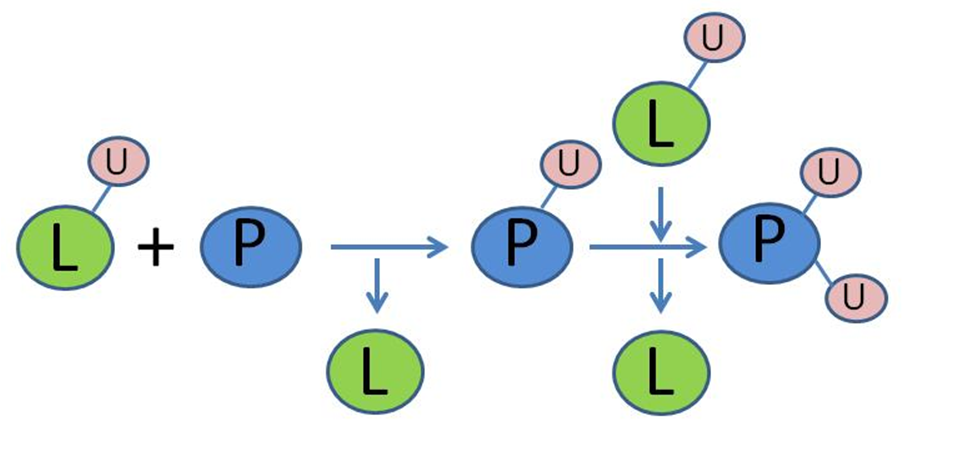
\includegraphics[width=0.4\textwidth]{./images/multimodel.png}}
	
	\subfloat[Cartoon representation of distributive polyubiquitination]{\label{fig:distrocartoon}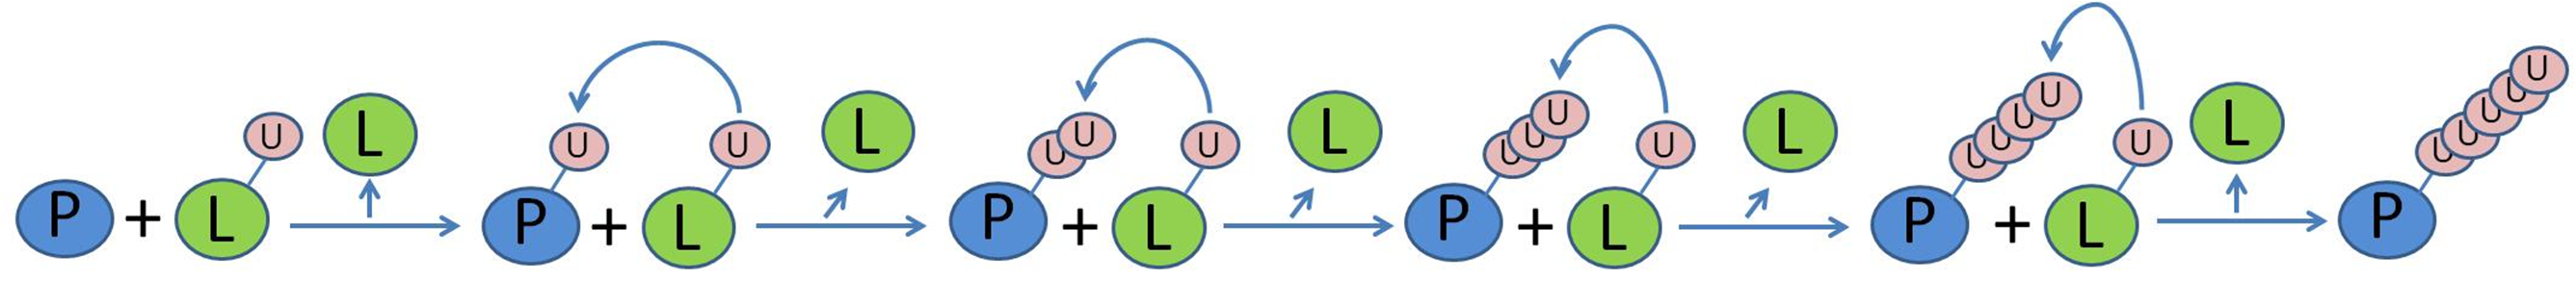
\includegraphics[width=1\textwidth]{./images/distmodel.png}}

	\subfloat[Cartoon representation of processive polyubiquitination]{\label{fig:proccartoon}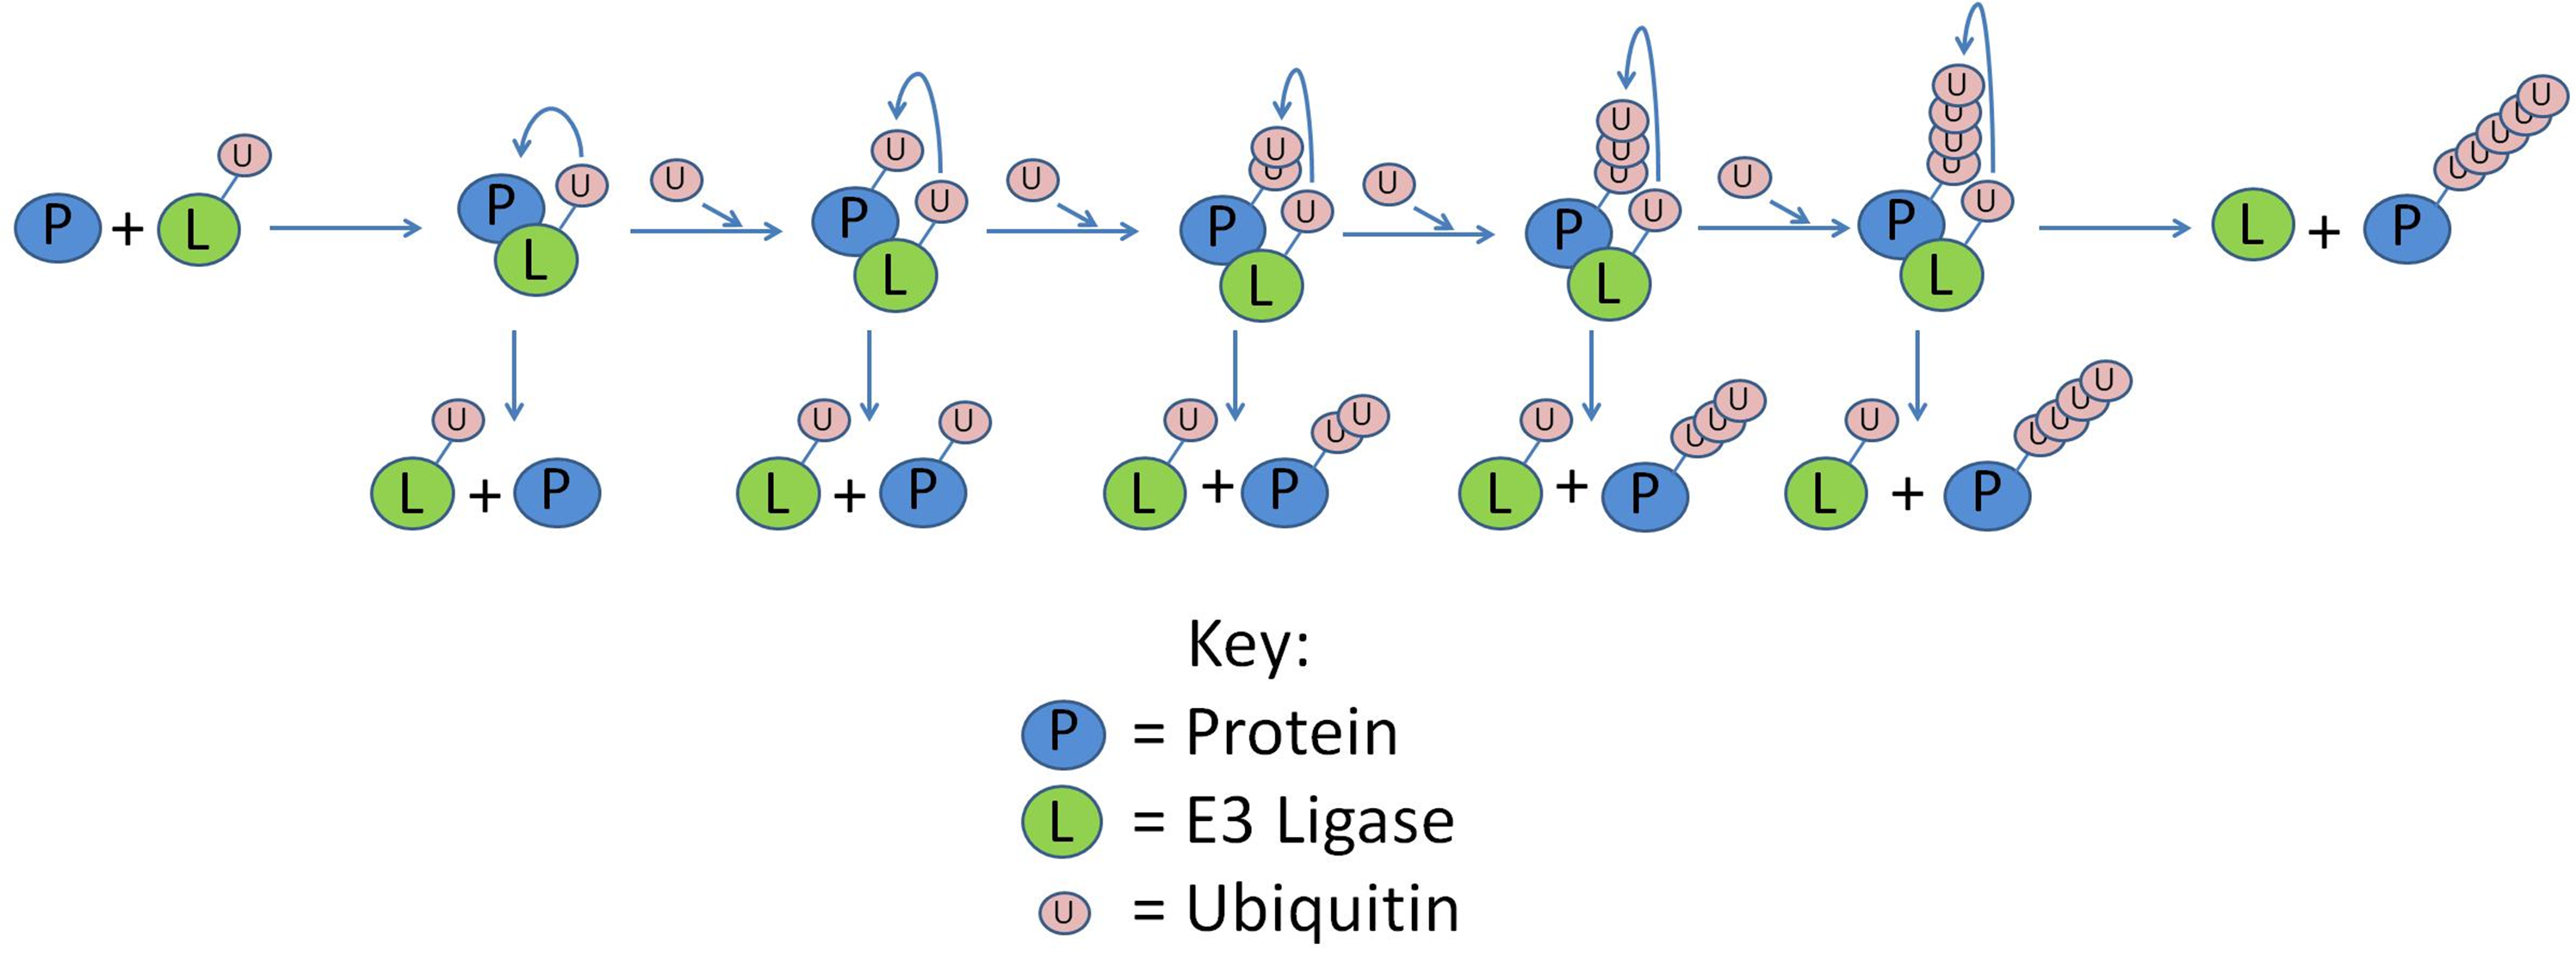
\includegraphics[width=1\textwidth]{./images/procmodel.png}}
	
	\caption{Cartoon representations of ubiquitination. A) is multiubiquitination, in which the protein is ubiquitinated at two different sites. B) is distributive polyubiquitination, in which the protein P is polyubiquitinated in a process involving multiple association and dissociation steps between the protein and the ligase L. C) is processive polyubiquitination, in which the protein P is polyubiquitinated in a process involving a single association event involving the protein and the ligase L.}
	\label{fig:ubi cartoon}
\end{figure}
}
%important to plants
%what is ubiquitination
Ubiquitin is a very stable 76 amino acid protein with a very strongly conserved structure through evolution\cite{vijay1987structure} which is present in all eukaryotic cells\cite{schlesinger1975complete}. When all ubiquitin-coding genes were deleted in \emph{Saccharomyces cerevisiae}, the result was a complete loss of viability\cite{finley1994inhibition}. This demonstrates how essential ubiquitin is for eukaryotic life. Ubiquitin has four exposed lysine residues, allowing it to covalently bond with other proteins. Ubiquitination is the covalent attachment of ubiquitin monomers, via the protruding C-terminus, to residues of a substrate protein by a ligase. Polyubiquitin chains form through the sequential addition of ubiquitin monomers to ubiquitins that are already attached to a protein substrate. 

Polyubiquitination is a post-translational modification which is vital for regulating protein function and degradation and plays a role in many cellular processes such as regulation of cell-cycle progression, transcription activity, signal transduction, antigen processing, apoptosis, chromatin structure and internalisation of receptors leading to their degradation\cite{hershko1998ubiquitin}. Processes such as the cell cycle are regulated by a series of protein degradation events\cite{bastians1999cell,glotzer1991cyclin}. Such is the importance of ubiquitination that it has been implicated in multiple diseases. Ubiquitination is important in cancer as it can regulate the cell cycle, the balance between proliferation and apoptosis, and autophagy\cite{kirkin2011ubiquitin}. Ubiquitination has also been linked to neurodegenerative diseases as it effects synaptic plasticity and the buildup of protein aggregates\cite{tai2008ubiquitin}.

Ubiquitination is important in plant molecular biology. Auxin is a plant hormone which is involved in most aspects of plant growth and development\cite{stewart2010trees}. Ubiquitination of transcriptional repressors in response to auxin signalling is a vital mode of action in plant development\cite{kelley2012ubiquitin}. Jasmonate is important in regulation of plant development and response to environmental pressures\cite{kombrink2012chemical}. A jasmonate receptor coronatine-insensitive1 is important in the degradation of some transcriptional repressors in response to jasmonate\cite{sheard2010jasmonate} via the ubiquitin pathway.

%how does it happen
Ubiquitination involves three enzymes. The ubiquitin-activating enzyme (E1) activates ubiquitin in an ATP-dependent manner. The ubiquitin-conjugating enzyme (E2) accepts the activated ubiquitin from E1. Activated ubiquitin is attached to the substrate in an E3 ligase-mediated fashion\cite{hershko1983components}. 

%importance of multiubiquitination
Ubiquitination can occur in multiple ways. For example, a single lysine of a protein can have a chain of ubiquitin monomers attached to it in polyubiquitination. Attachment of ubiquitin chains is vital for proteolysis as the ubiquitinated protein is targeted for degradation by the proteosome\cite{finley1994inhibition,ciechanover1984ubiquitin,emmerich2011emerging}. Polyubiquitination can occur in a processive or distributive manner\cite{rape2006processivity}. Processive polyubiquitination involves the serial addition of ubiquitin to a growing chain while the ligase remains bound to the substrate protein. Conversely during distributive polyubiquitination the ligase releases the substrate after the addition of each ubiquitin monomer. Multiubiquitination is the addition of single ubiquitin monomers to multiple sites of the same protein. This often occurs on receptor proteins and leads to their internalisation and lysosomal degradation\cite{monami2008grb10,staub2006role,mosesson2003endocytosis,haglund2003multiple}. These processes are illustrated in figure~\ref{fig:ubi cartoon}.

Recent evidence has suggested that chains of ubiquitin are built up in a stepwise fashion and are not passed to the substrate protein fully formed as was previously believed\cite{li2007ubiquitin}. This was discovered by Pierce et al\cite{pierce2009detection} following the development of a new experimental technique which allows the ubiquitination process to be followed on a millisecond timescale which was not previously possible. This technique allowed intermediates during the buildup of polyubiquitin chains to be captured and analysed, showing that the chains are built up in a stepwise fashion and not transferred whole to the substrate protein. This development will allow ubiquitination to be studied in more depth experimentally, which was previously challenging as ubiquitination occurs over a short timescale.

Polyubiquitination determines the substrate ordering of anaphase-promoting complex (APC) substrates. Substrates are polyubiquitinated in a well defined order by the APC. The complex sequence of protein ubiquitinations is termed substrate ordering and is required for proper cellular function. In 2006, Rape et al\cite{rape2006processivity} showed that the substrate ordering is determined by the processivity of the substrate: proteins are ubiquitinated according to where they sit on a continuum between processive and distributive polyubiquitination. Their processivity has implications for how the proteins compete for the ligase. Processively polyubiquitinated proteins bind the ligase once to achieve polyubiquitination, whereas distributively polyubiquitinated proteins must rebind the ligase multiple times to become polyubiquitinated. This means that processively polyubiquitinated proteins will outcompete distribuitively polyubiquitinated proteins and so are ubiquitinated more rapidly. Examples of processive proteins are securin and geminin. They are degraded in the presence of low concentrations of the ligase UbcH10 because they only need to bind the ligase once. Cyclin A is not degraded in the presence of low concentrations of UbcH10\cite{rape2004autonomous} as it is outcompeted for binding by the more processive proteins securin and geminin. Rapid degradation is due to more processive ubiquitination. The position of the protein on the processivity scale determines the speed at which substrate is degraded and defines the substrate ordering.

%why model
The pace of the ubiquitination process, along with its complexity at the molecular level, makes it challenging to study \emph{in vitro} or \emph{in vivo}. Coupled with its emerging clinical significance, this makes the process a suitable candidate for investigation by mathematical modelling. The development of a simplified model of the process will improve our understanding of this complex process and may allow the the mode of ubiquitination to be determined from experimental results. Modelling the process will also improve our understanding of which rate constants are important. Rate constants control the rates of reaction and one step may control the whole process. This is named the rate limiting step, and is often of therapeutic importance: by targeting the rate limiting step a process can be sped up or inhibited, with therapeutic implications. 

%what we intend to do
This study will aim to create a novel series of models of ubiquitination. Multiubiquitination and polyubiquitination will be modelled by creating a series of ordinary differential equations (ODEs) describing the processes. These ODEs will be solved computationally, and the results will be plotted. The plots will be analysed and compared to find the implications for our understanding of ubiquitination.


\section{Methods and Materials}

The method used to generate the models is best described using the example process of an enzyme (E) binding to its substrate (S) to form the enzyme-substrate complex (ES) which reacts to form the product (P) and E. This is shown below:

\begin{equation}
  E + S \xrightleftharpoons[k_\text{off}]{k_\text{on}} ES
  \xrightarrow[{}]{k_\text{cat}} E + P
\end{equation}

This process can be described as a series of ODEs, which describe the rate of change of the concentration of each species as a function of the concentrations of all species. The ODEs for this process are shown below:
\begin{align}
 \frac{\delta E}{\delta t} &= k_\text{off}[ES] + k_\text{cat}[ES] - k_\text{on}[E][S] \\
 \frac{\delta S}{\delta t} &= k_\text{off}[ES] - k_\text{on}[E][S] \\
 \frac{\delta ES}{\delta t} &= k_\text{on}[E][S] - k_\text{off}[ES] - k_\text{cat}[ES] \\
 \frac{\delta P}{\delta t} &= k_\text{cat}[ES]
\end{align}

These ODEs can be numerically solved to give information on the process. This approach was followed to create models of the more complex ubiquitination pathways investigated.

The Python language \cite{Rossum:1995:PRM:869369} and the SciPy toolkit \cite{scipy2001} was used to numerically solve the models using the odeint module. 2D plots were created using the matplotlib module of Python (see figure~\ref{fig:multi model}). MATLAB\cite{MATLAB:2010} was used to create 3D plots of data generated in Python (see figure~\ref{fig:Sampling}).

\section{Results}

\subsection{Modelling Multiubiquitination}\label{multi}
%\afterpage{
\begin{figure}[H]
	\centering
	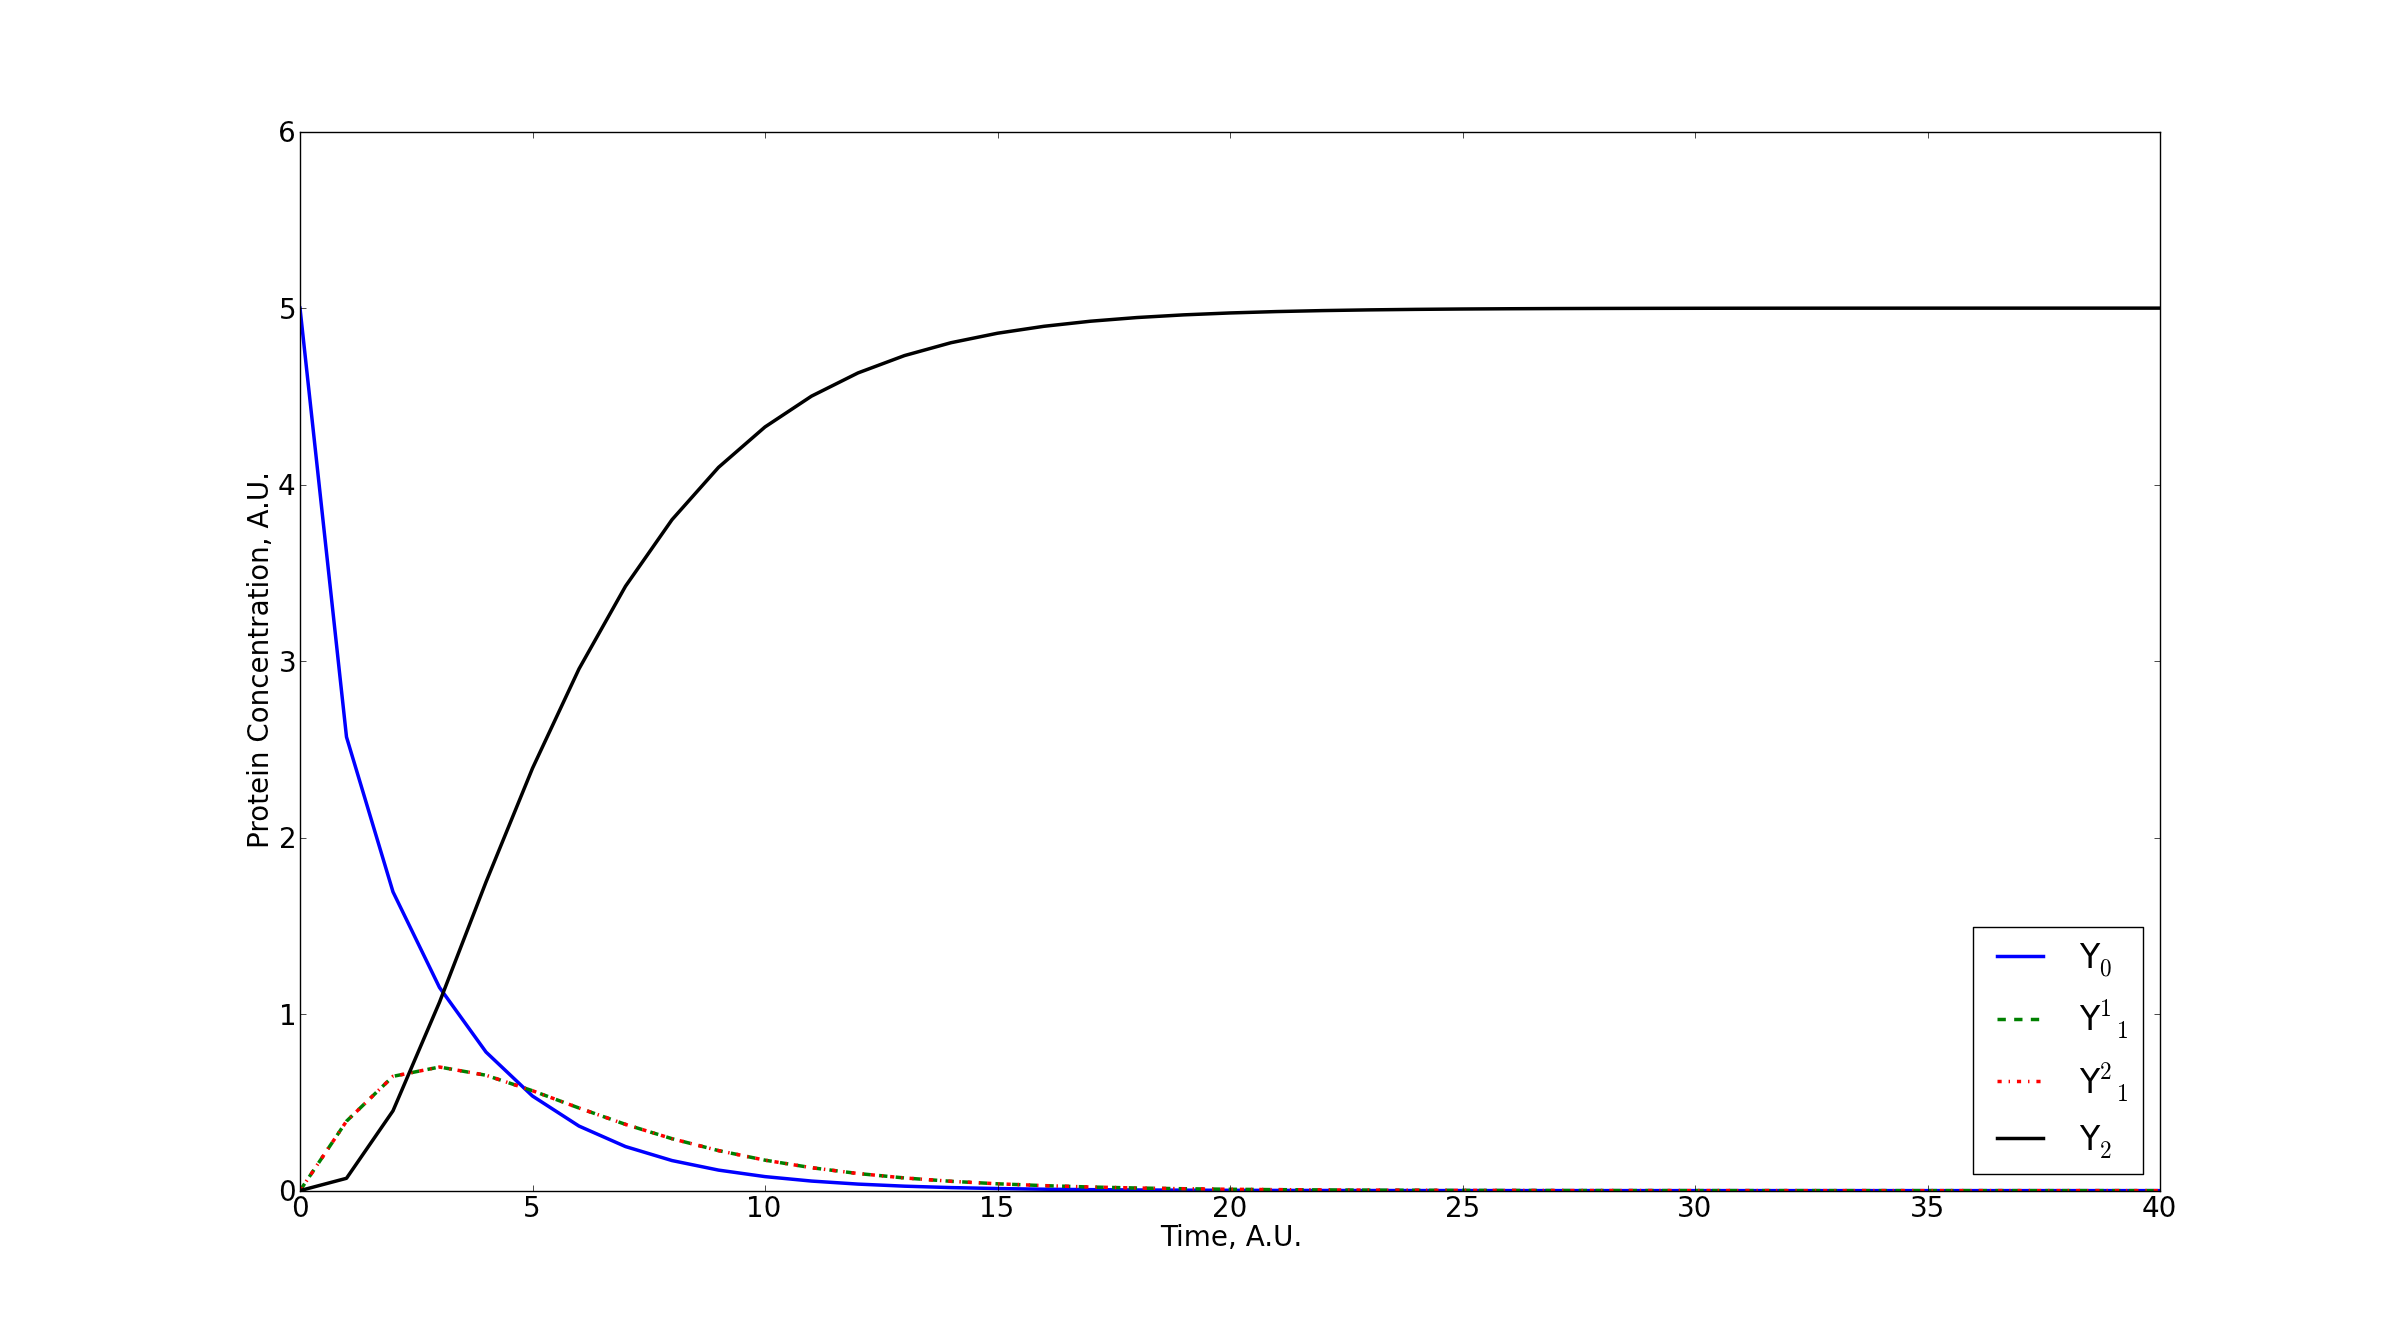
\includegraphics[width=1.0\textwidth]{./images/simple_multimodel.png}
	\caption{Numerical solutions to our model of multiubiquitination for species Y$_0$, Y$^1$$_1$, Y$^2$$_1$ and Y$_2$, defined in appendix 1. The model (see appendix 1) consist of a series of ordinary differential equations which were numerically solved. Here, all rate constants were set at 1 except k$_2$ and k$_6$ which were both 0.5.}
	\label{fig:multi model}
\end{figure}
%}

Multiubiquitination involves the covalent attachment of single ubiquitin monomers to two different sites on a target protein by an E3 ligase. The cartoon in figure~\ref{fig:multicartoon} demonstrates an example of this. The corresponding mathematical model is given in appendix 1. This model was numerically solved. The resulting series of concentrations were plotted against time. This is shown in figure~\ref{fig:multi model}.

Over time, the concentration of the initial substrate decreases rapidly to zero. The intermediate monoubiquitinated proteins initially increase however their concentration slowly decreases to zero as these species are used up in the formation of the multiubiquitinated final product. Both monoubiquitinated proteins have an identical profile here, as the rate constants k$_2$ and k$_6$ which control their formation are equal. If the rate constants were altered, the profiles of the intermediates would change however they would both decrease to zero by the end of the simulation. The final product increases in concentration over time until its concentration is equal to the concentration of protein added to the system. No other species are present at the end of the model.

\subsection{Polyubiquitination}

\afterpage{
\begin{figure}[H]
	\centering
	\subfloat[Numerical evaluation of a model of distributive polyubiquitination]{\label{fig:Distributive Polyubiquitination}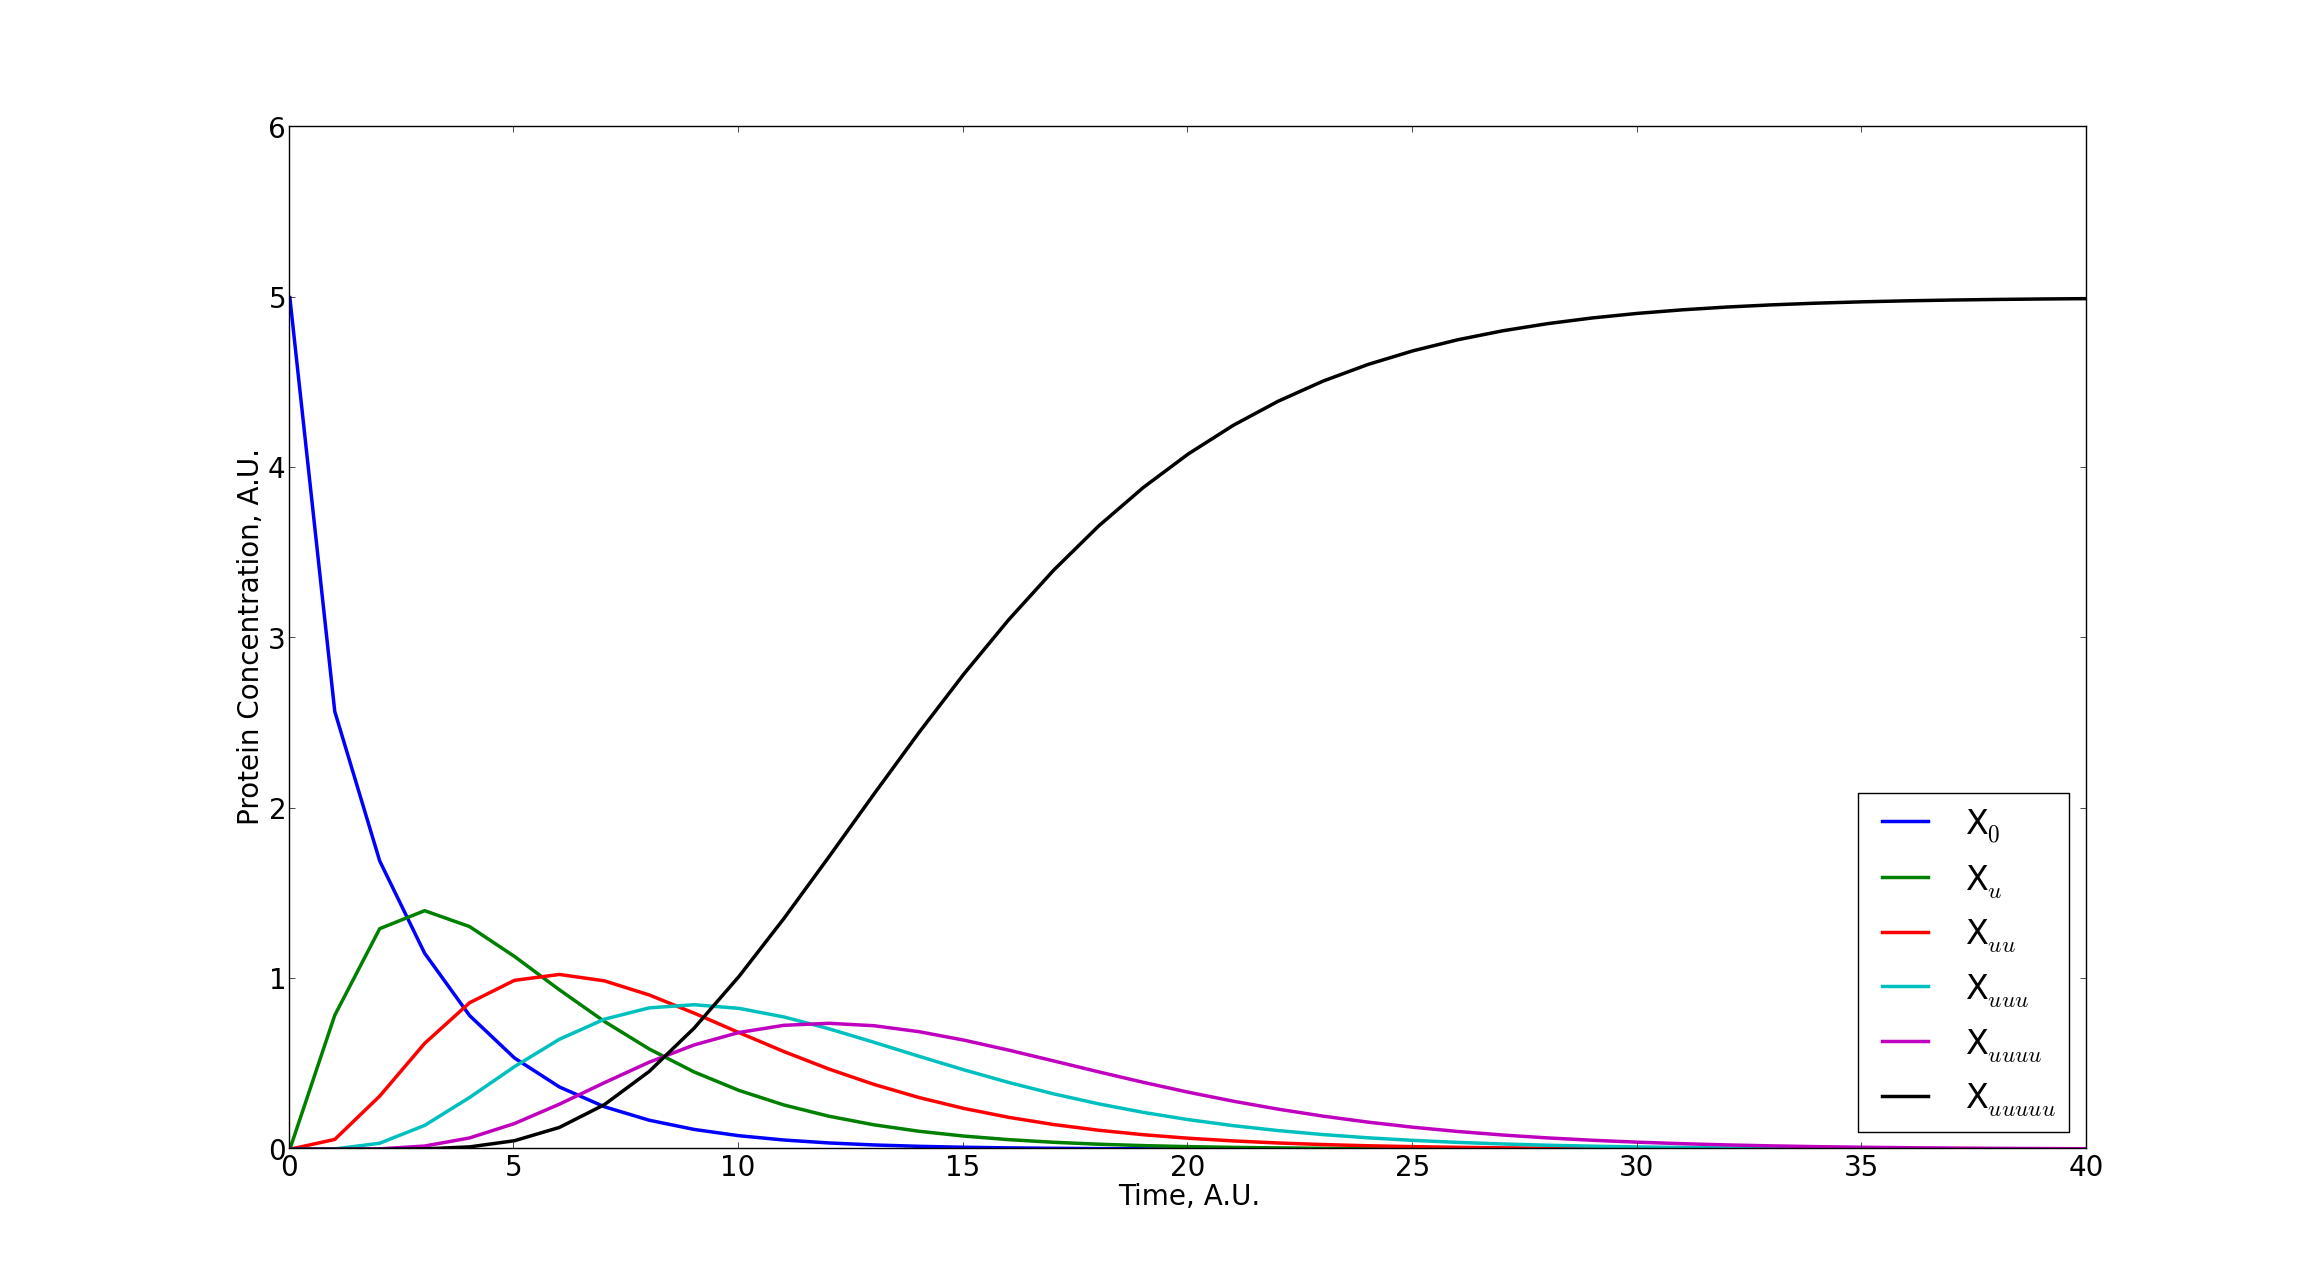
\includegraphics[width=1.0\textwidth]{./images/simplepolydist.png}}
	
	\subfloat[Numerical evaluation of a model of processive polyubiquitination]{\label{fig:Processive Polyubiquitination}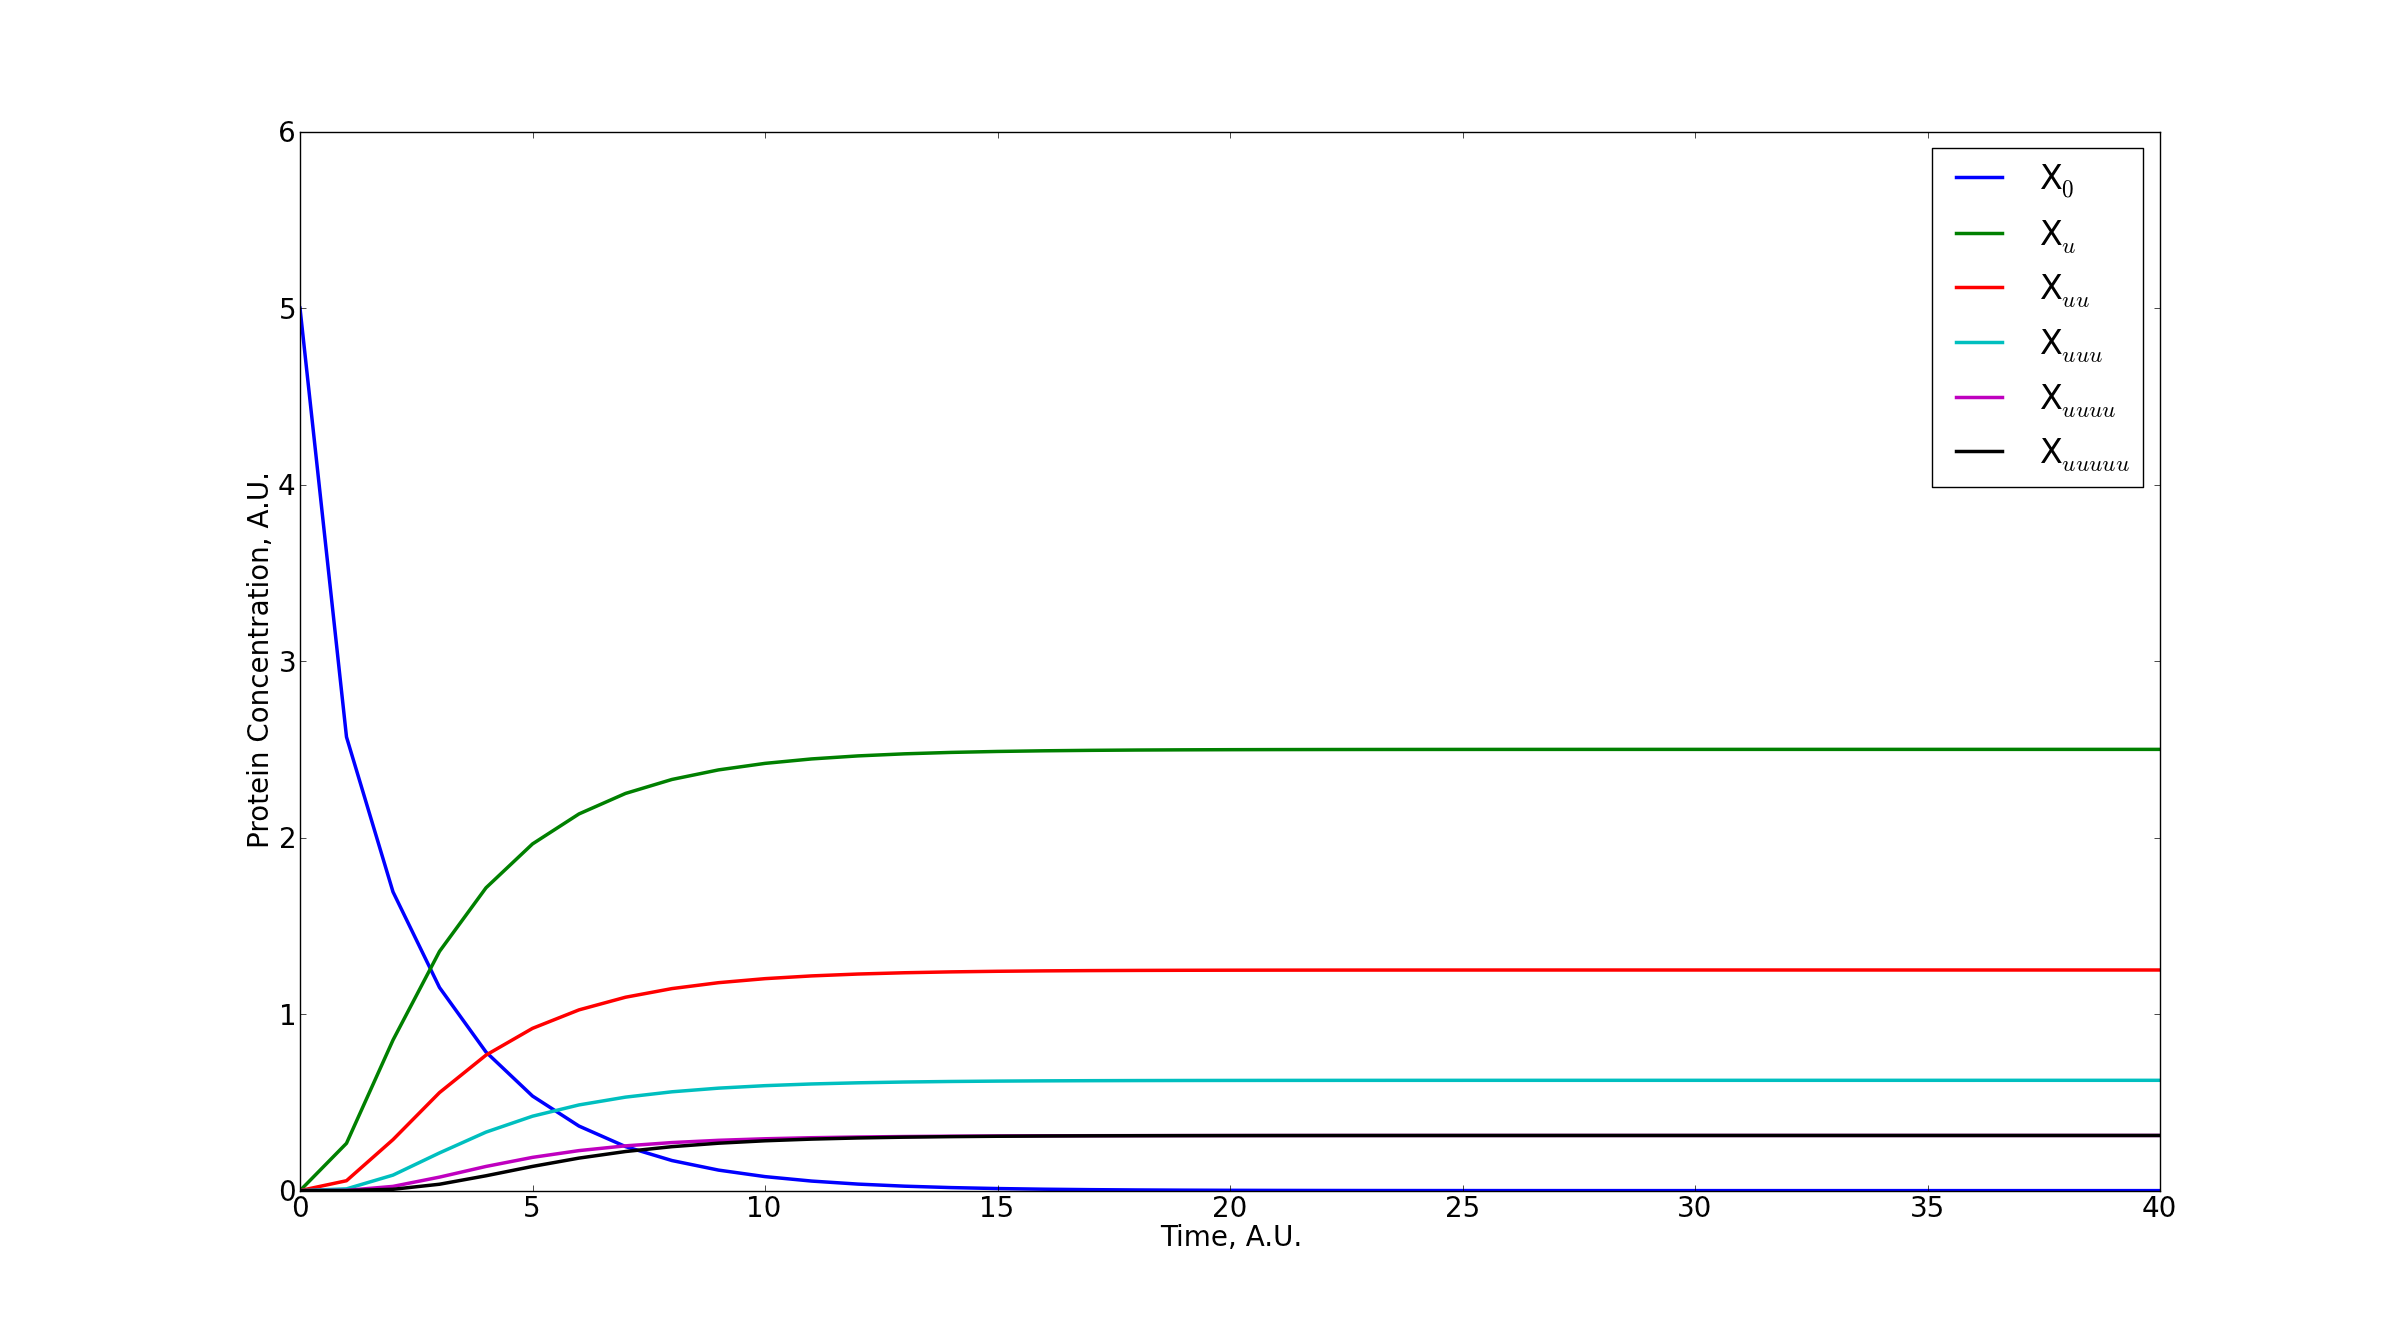
\includegraphics[width=1.0\textwidth]{./images/processivepoly.png}}

	\caption{Numerical solutions to models of processive and distributive polyubiquitination for species X$_0$, X$_u$, X$_{uu}$, X$_{uuu}$, X$_{uuuu}$ and X$_{uuuuu}$ defined in appendix 2. Models shown in appendices 2 and 3, respectively, were numerically solved. The results of the models were plotted against time. Here, all the rate constants were set at 1.}
	\label{fig:Polyubiquitination models}
\end{figure}
}

Polyubiquitination is the formation of a chain of covalently bonded ubiquitin monomers on one lysine residue of the substrate protein. We considered two mechanisms for polyubiquitination: distributive polyubiquitination (see figure~\ref{fig:distrocartoon}) and processive polyubiquitination (see figure~\ref{fig:proccartoon}). In distributive polyubiquitination, the addition of a ubiquitin monomer to the growing chain occurs following the association of the protein with a ligase. This complex dissociates after the monomer is added to the chain. This contrasts with processive polyubiquitination in which the protein stays associated with the same E3 ligase enzyme throughout the formation of the ubiquitin chain. The ligase and substrate protein may dissociate during the process however they do not reassociate. We determined to create abstract models of these processes.

\subsubsection{Distributive Polyubiquitination}\label{distro}

The model of distributive polyubiquitination is given in appendix 2. The model was numerically solved. The results were plotted against time and can be seen in figure ~\ref{fig:Distributive Polyubiquitination}. Over time, the concentration of the initial substrate decreased rapidly to zero. Concentration of the intermediate species sequentially increased and decreased. The concentration of the polyubiquitinated protein X$_{uuuuu}$ increased in a sigmoidal fashion until it reached 5 A.U., the starting concentration of unubiquitinated protein X$_0$. No other species were present at the end of the simulation. In order to compare the behaviour of distributive and processive polyubiquitination, processive polyubiquitination was modelled.

\subsubsection{Processive Polyubiquitination}\label{proc}

The model of processive polyubiquitination is given in appendix 3. It has a constant k$_\text{off}$ rate. The model was numerically solved. The results were plotted against time and are shown in figure~\ref{fig:Processive Polyubiquitination}. The concentration of the initial substrate X$_0$ decreased rapidly to zero. The concentration of the other species increased and plateaued at sequentially lower concentrations. The end levels of each species can be altered by changing the rates of reaction (data not shown). The processive model reached thermodynamic equilibrium after between 10 and 15 A.U., which was much faster than the distributive model which reached equilibrium after between 35 and 40 A.U.

\subsubsection{Comparison to Experimental Results}

\afterpage{
\begin{figure}[H]
	\centering
	\subfloat[Comparison of a numerically solved model of processive polyubiquitination with experimentally derived values of $\beta$-Cat polyubiquitination]{\label{fig:bcat v model}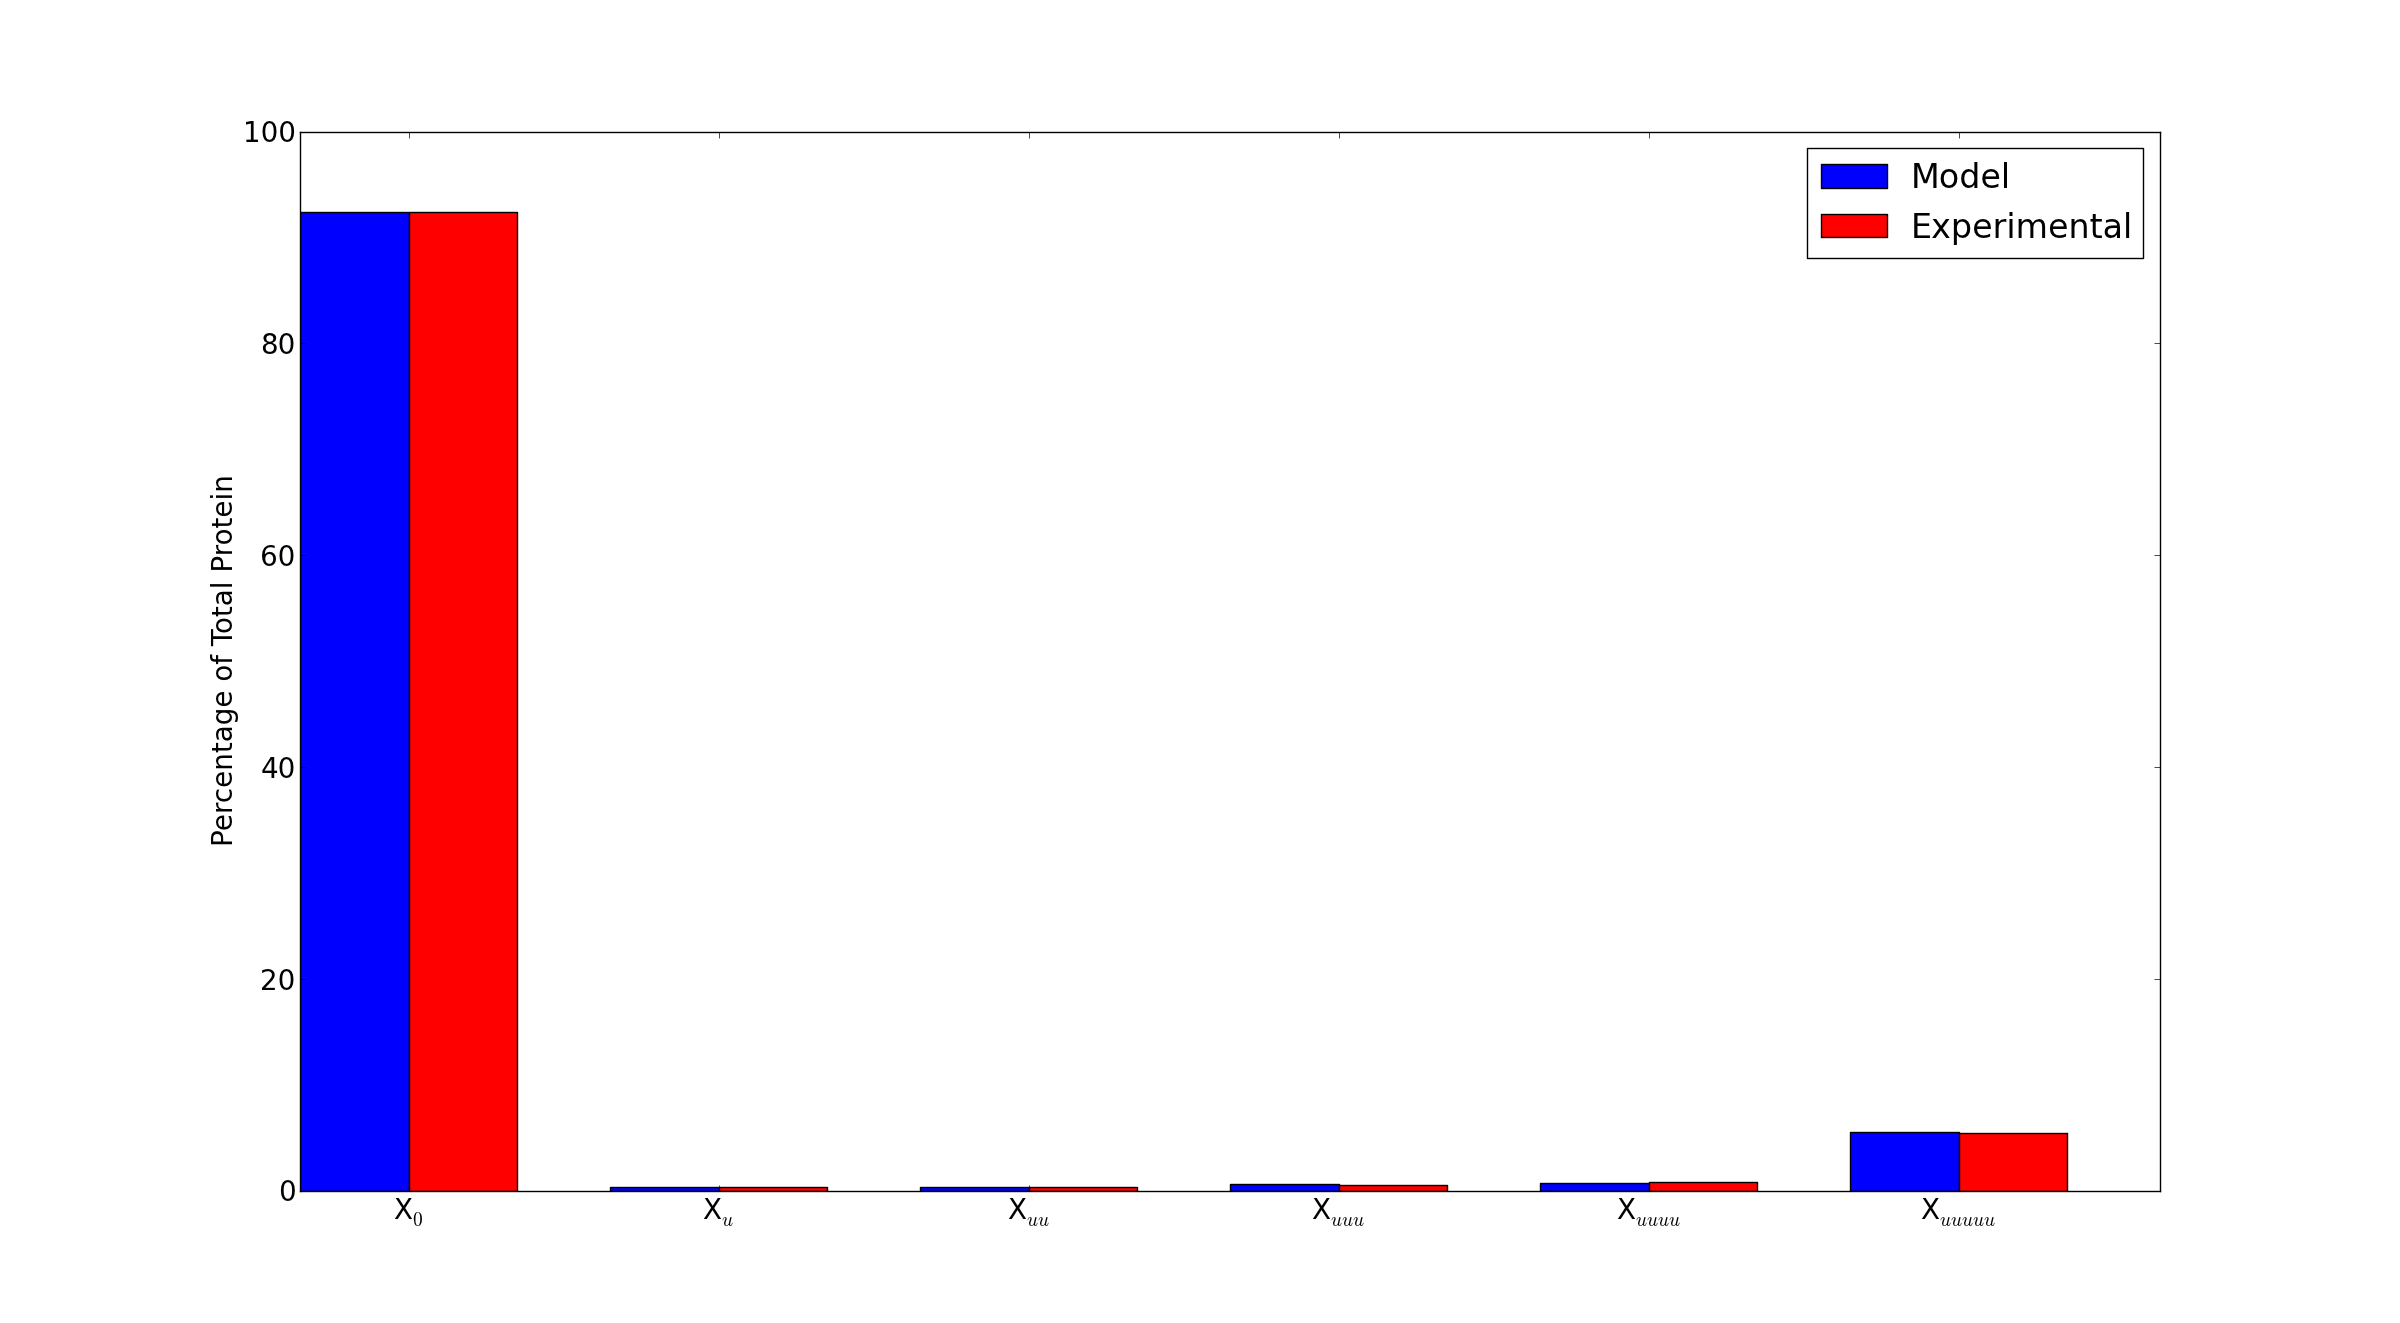
\includegraphics[width=1.0\textwidth]{./images/bar_chartbcat.png}}

	\subfloat[Comparison of a numerically solved model of processive polyubiquitination with experimentally derived values of CYCE polyubiquitination]{\label{fig:cyce v model}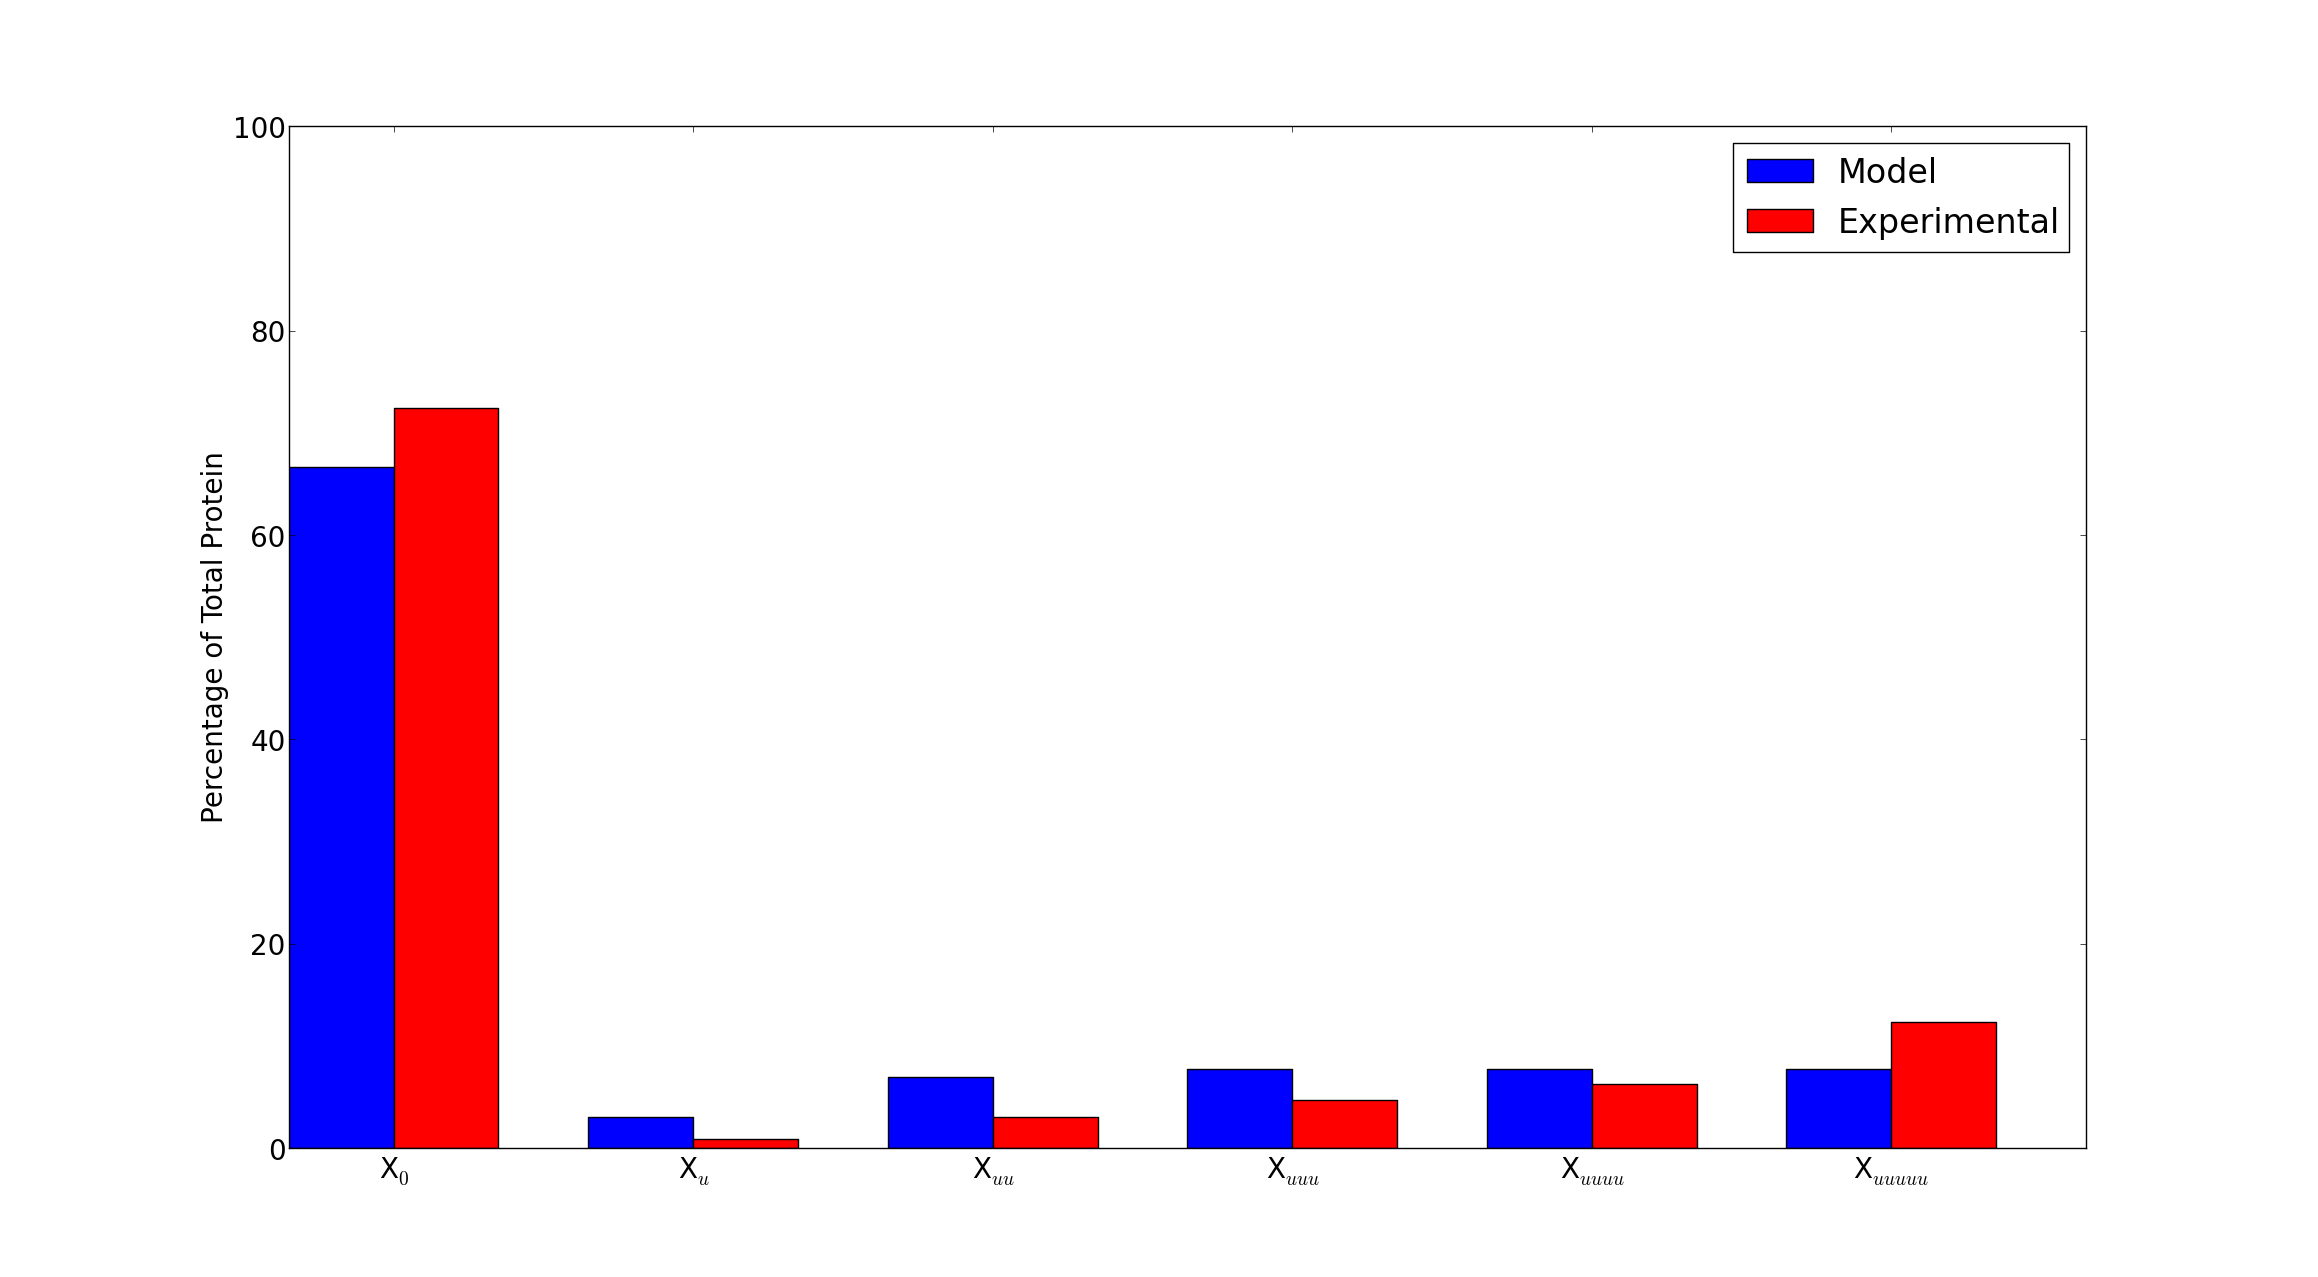
\includegraphics[width=1.0\textwidth]{./images/bar_chart_cyce.png}}

	\caption{Comparison of experimentally determined results with predicted results from numerical evaluation of a processive polyubiquitination model. Plots show experimentally determined concentrations of proteins in different ubiquitinaion states at the end of the given reaction period. The model of processive polyubiquitination was adapted to reflect the \emph{in vitro} experimental work carried out by Pierce et al.\cite{pierce2009detection}. The experimentally determined rate constants were used in the models, which were evaluated. The final concentrations of each species were plotted and compared to the experimentally determined final concentration. Note that the model's final species is X$_{uuuuu}$ whereas the experimental system ran to X$_{uuuuuuuuu}$ and so the X$_{uuuuu}$ term for the experimental data is the sum of the concentrations of X$_{uuuuu}$ onwards.}
	\label{fig:model v experimental}
\end{figure}
}

Recently, Pierce et al \cite{pierce2009detection} developed a new technique to allow the determination of the rate constants and final levels of the species involved in an \emph{in vitro} polyubiquitination model. In this paper, the polyubiquitination of $\beta$-Cat and CYCE were investigated and were determined to display processive polyubiquitination. 

In order to validate the model we developed, the rate constants from the paper were used in our processive polyubiquitination model. In these simulations, the k$_\text{off 0}$ rate was set at 0 and a X$_0$.L concentration of 5 A.U. was used. These changes were made to reflect the \emph{in vitro} model used in the paper.

The modified models of processive polyubiquitination were numerically solved as before. The concentration of each species was plotted as a percentage of all species. Each species was plotted next to the experimentally determined value from the paper (figure ~\ref{fig:model v experimental}).  As the experimental system involved species with ubiquitin chains up to nine ubiquitins long, whereas our model only ran to five ubiquitins long, the experimental data at the point X$_{uuuuu}$ is the sum of the protein from X$_{uuuuu}$ to X$_{uuuuuuuu}$.

Pearson correlation coefficients\cite{pearson} were calculated for the data. For both proteins there was a strong correlation between the model and experimental data. The $\beta$-cat data had a P-value of 4.4195e-12 and the CYCE data had a P-value of 4.4860e-5. This shows that for both $\beta$-Cat and CYCE, there was no significant difference between our \emph{in silico} model predictions and the experimental \emph{in vitro} data from Pierce et al \cite{pierce2009detection}. This showed that this model of processive polyubiquitination can return the distribution of protein species at the end of a process, given the rate constants for that process.

This experiment showed that our model can produce a varied output. The general trend of our predictions matched the experimental data. The results were further fine tuned by the parameters which were experimentally determined. The disparity in CYCE results suggests that these parameters may not be correct.

\subsubsection{Unified Model of Polyubiquitination}\label{unifed}

Within polyubiquitination, it is known that there is a sliding scale of processivity between entirely processive and entirely distributive. This creates a mechanism for substrate ordering in late mitosis and G1, which is vital for regulating these processes \cite{rape2006processivity}. 

We modelled this sliding scale by altering the processive model of polyubiquitination. Following the dissociation of the ligase from the substrate, the species here can reassociate with the ligase and re-enter the pathway. In this scenario, the processive model has distributive characteristics and so is termed the unified model of polyubiquitination. This model is illustrated in figure~\ref{fig:Cartoon of Unified Polyubiquitination}. This was modelled (see appendix 4) and numerically solved. The results were plotted and can be seen in figure~\ref{fig:Unified Polyubiquitination}.

\afterpage{
\begin{figure}[H]
	\centering
	\subfloat[Cartoon of the unified model of polyubiquitination]{\label{fig:Cartoon of Unified Polyubiquitination}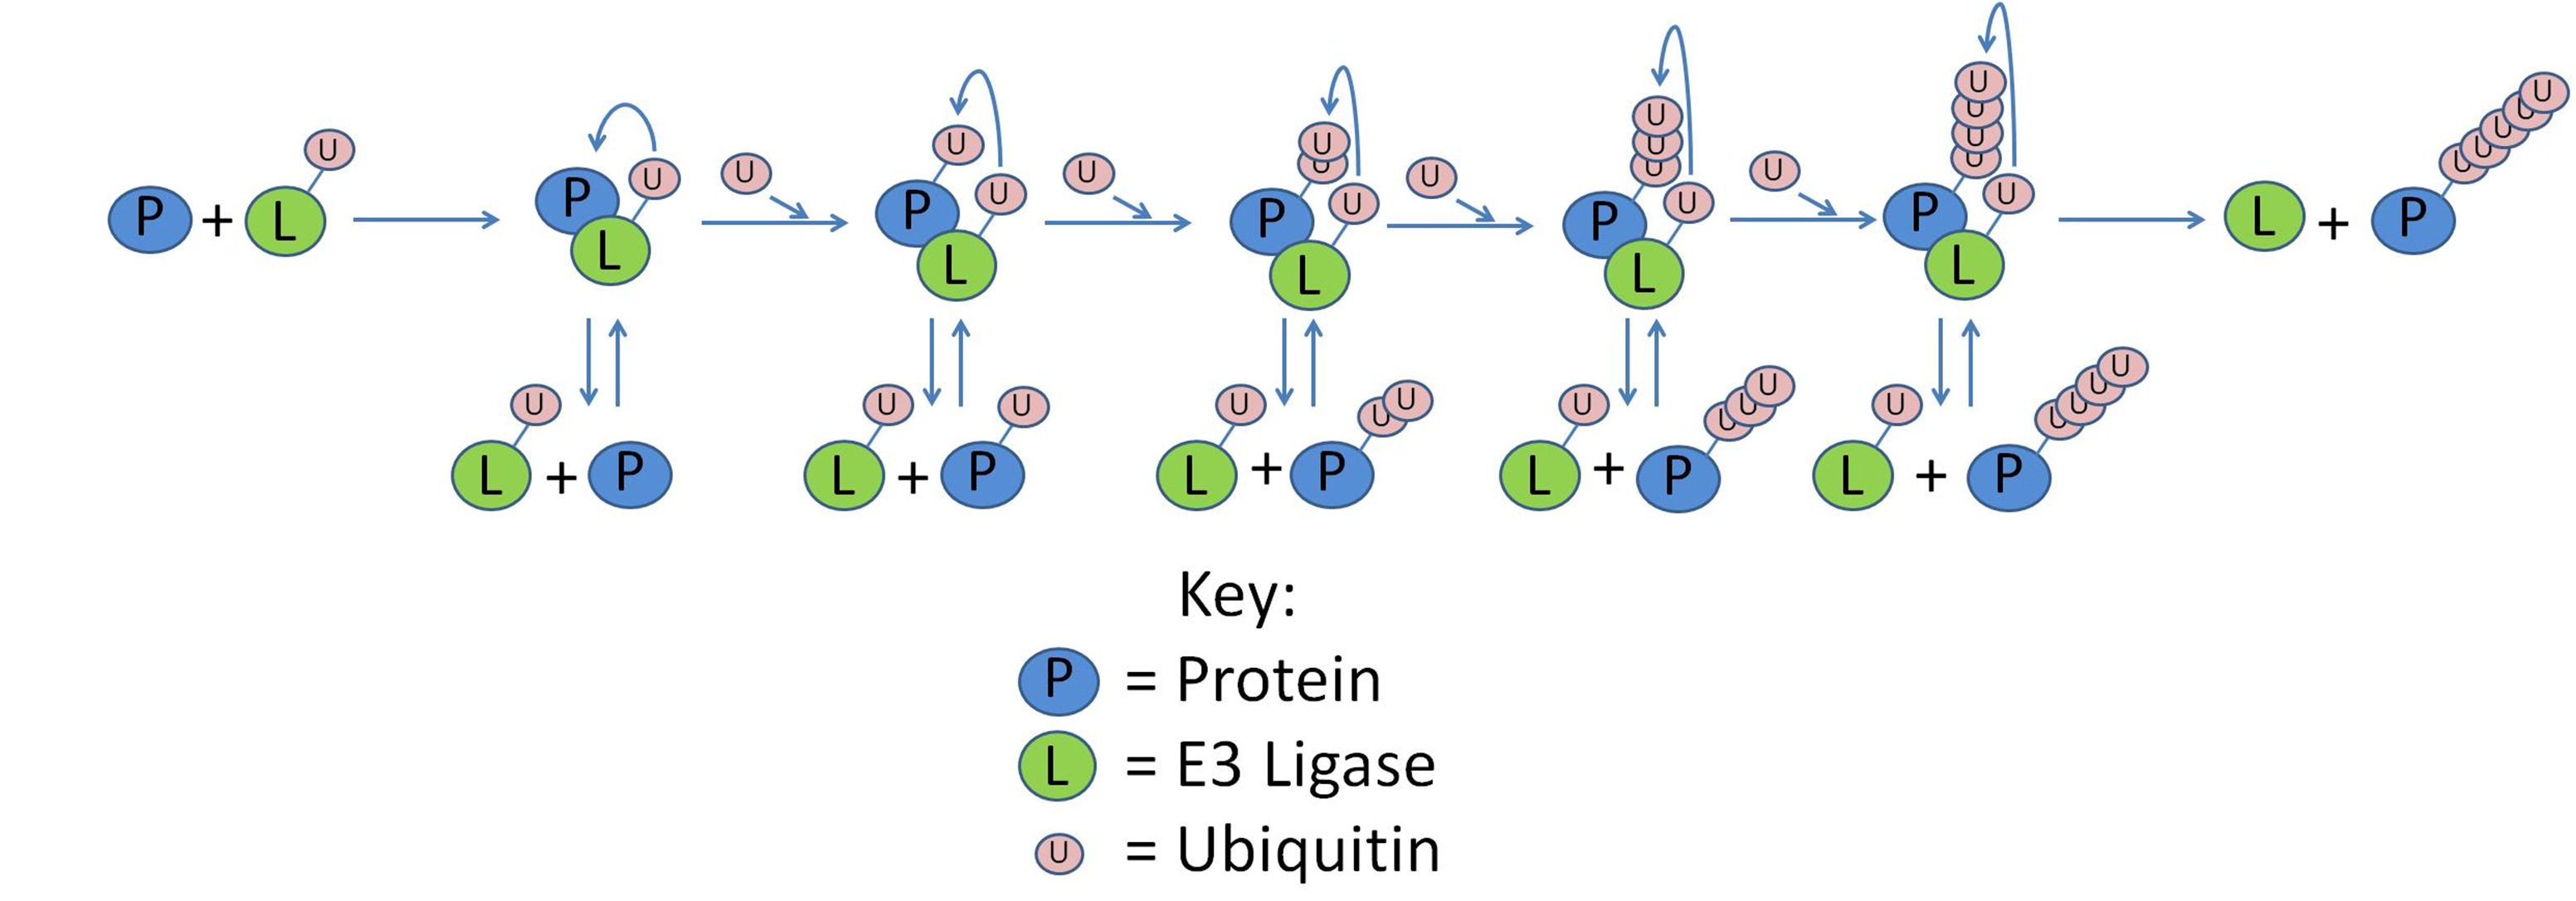
\includegraphics[width=1.0\textwidth]{./images/ubi_unified.png}}
	
	\subfloat[Numerical evaluation of a unified model of polyubiquitination]{\label{fig:Unified Polyubiquitination}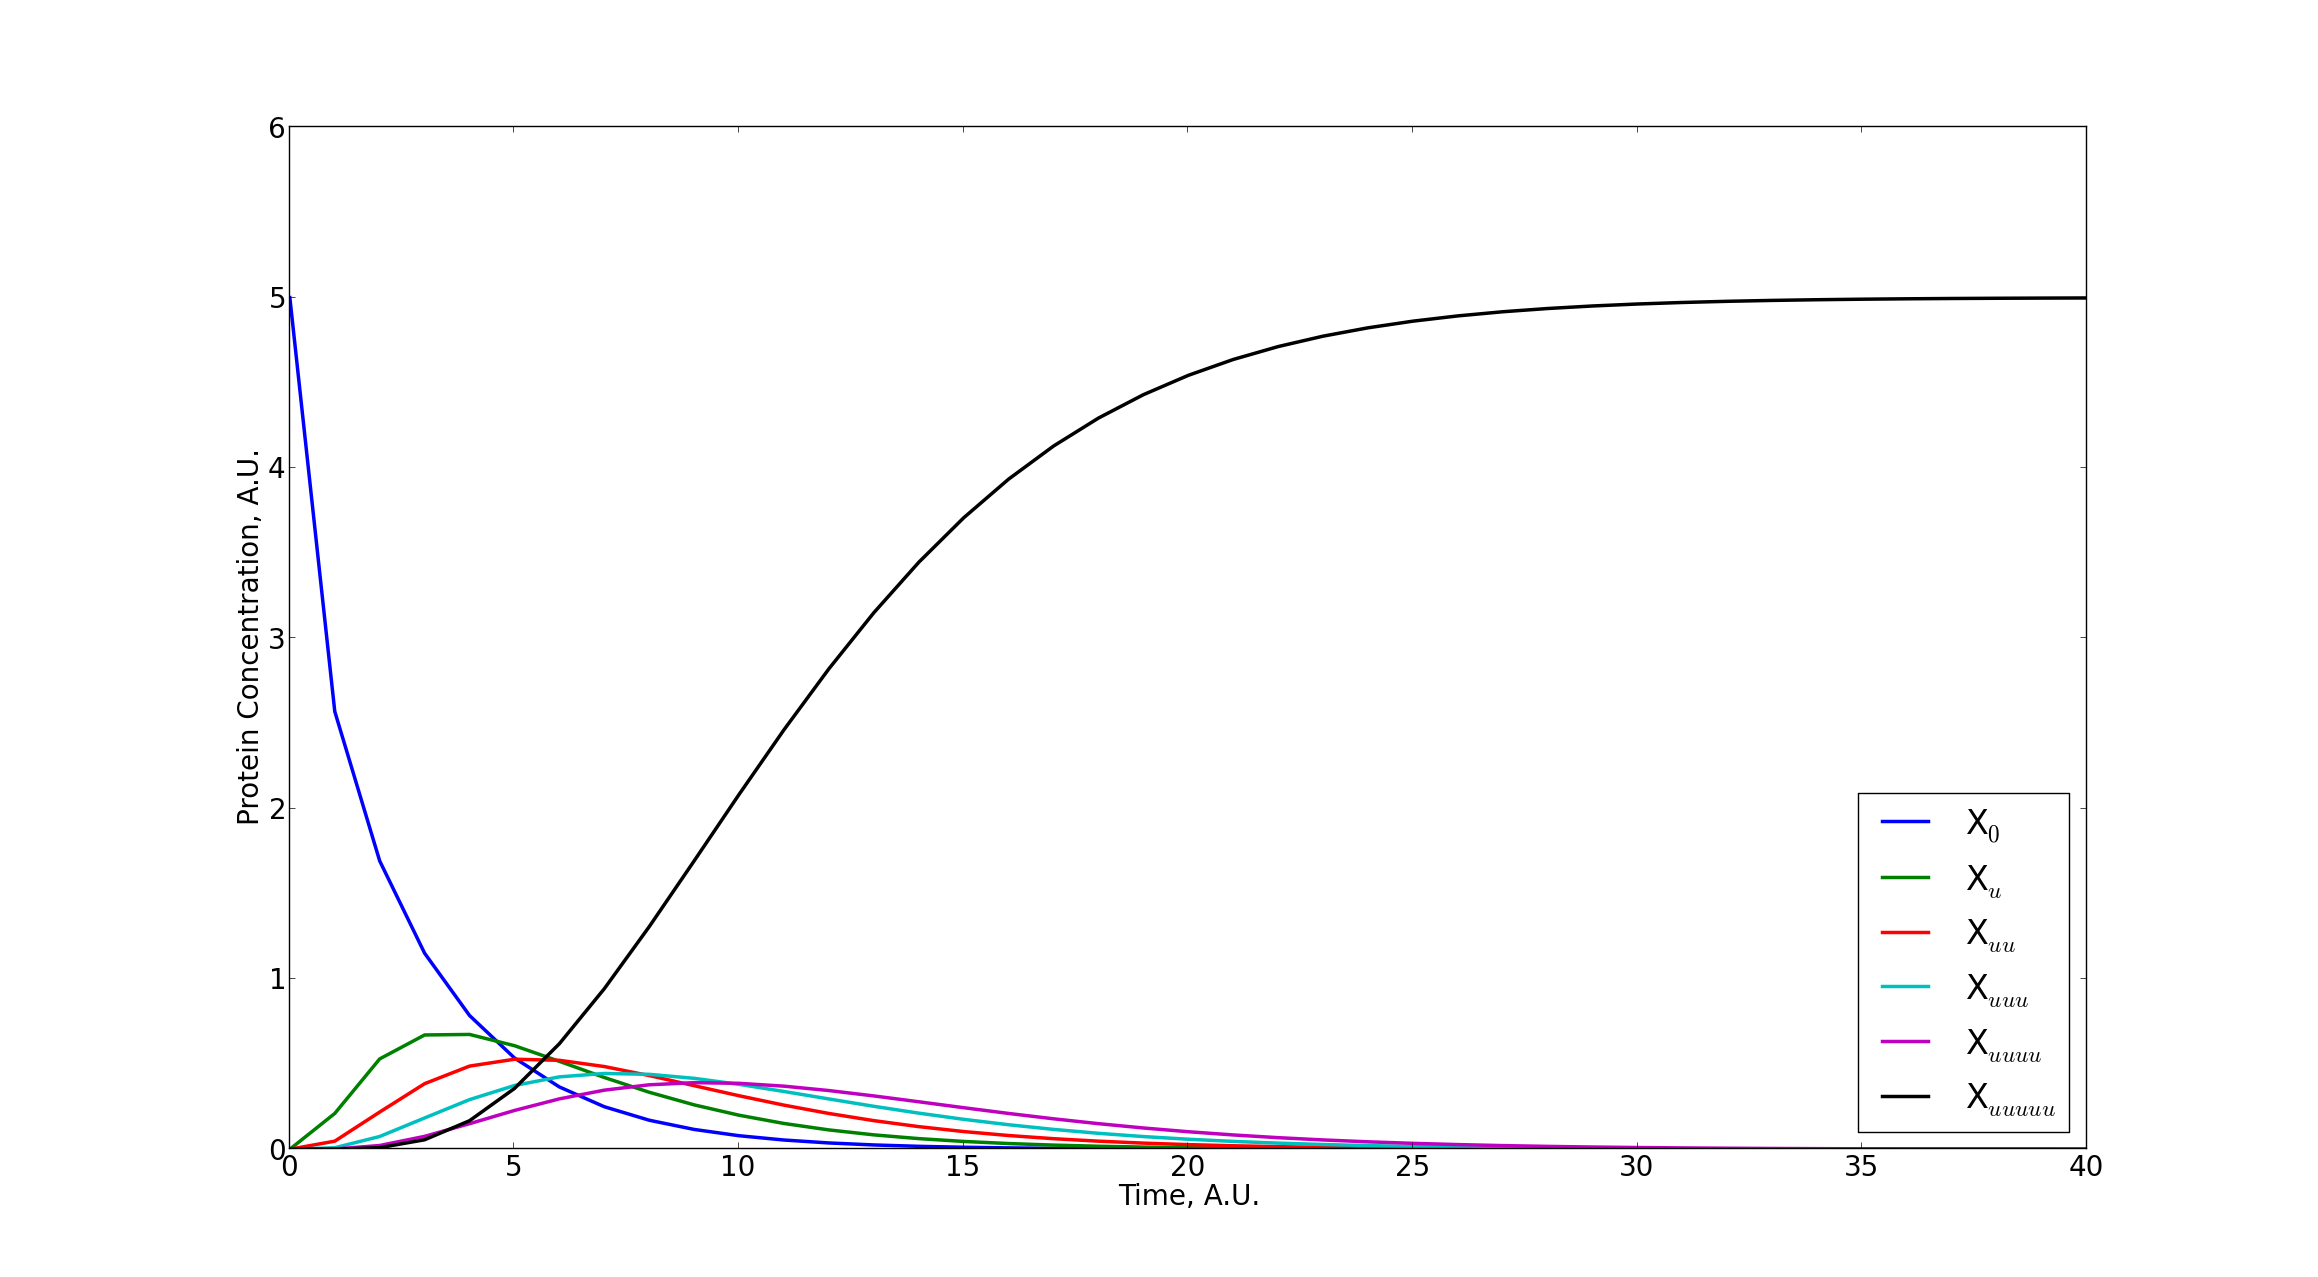
\includegraphics[width=1.0\textwidth]{./images/unified.png}}

	\caption{Cartoon and results of numerical evaluation of a unified model of polyubiquitination. Part a) shows a cartoon representation of the process. It demonstrates the option for intermediates to reassociate with the ligase to continue the process, which differentiates it from processive polyubiquitination. Part b) shows the results of the numerical evaluation of the model plotted against time. All rate constants were set at 1.}
	\label{fig:Unified model}
\end{figure}
}

The results of this simulation closely resemble those of the distributive polyubiquitination model (see figure~\ref{fig:Distributive Polyubiquitination}). The concentration of the initial substrate X$_0$ decreased rapidly to zero. The intermediate species sequentially increased before decreasing slowly to zero. Unlike the processive polyubiquitination model (see figure~\ref{fig:Processive Polyubiquitination}) intermediate species do not remain at the end of the simulation. The concentration of X$_{uuuuu}$ increased in a sigmoidal fashion. At the end of the simulation, only X$_{uuuuu}$ was present in the system. 

\subsection{Predicted Western Blot}

\afterpage{
\begin{figure}[H]
	\centering
	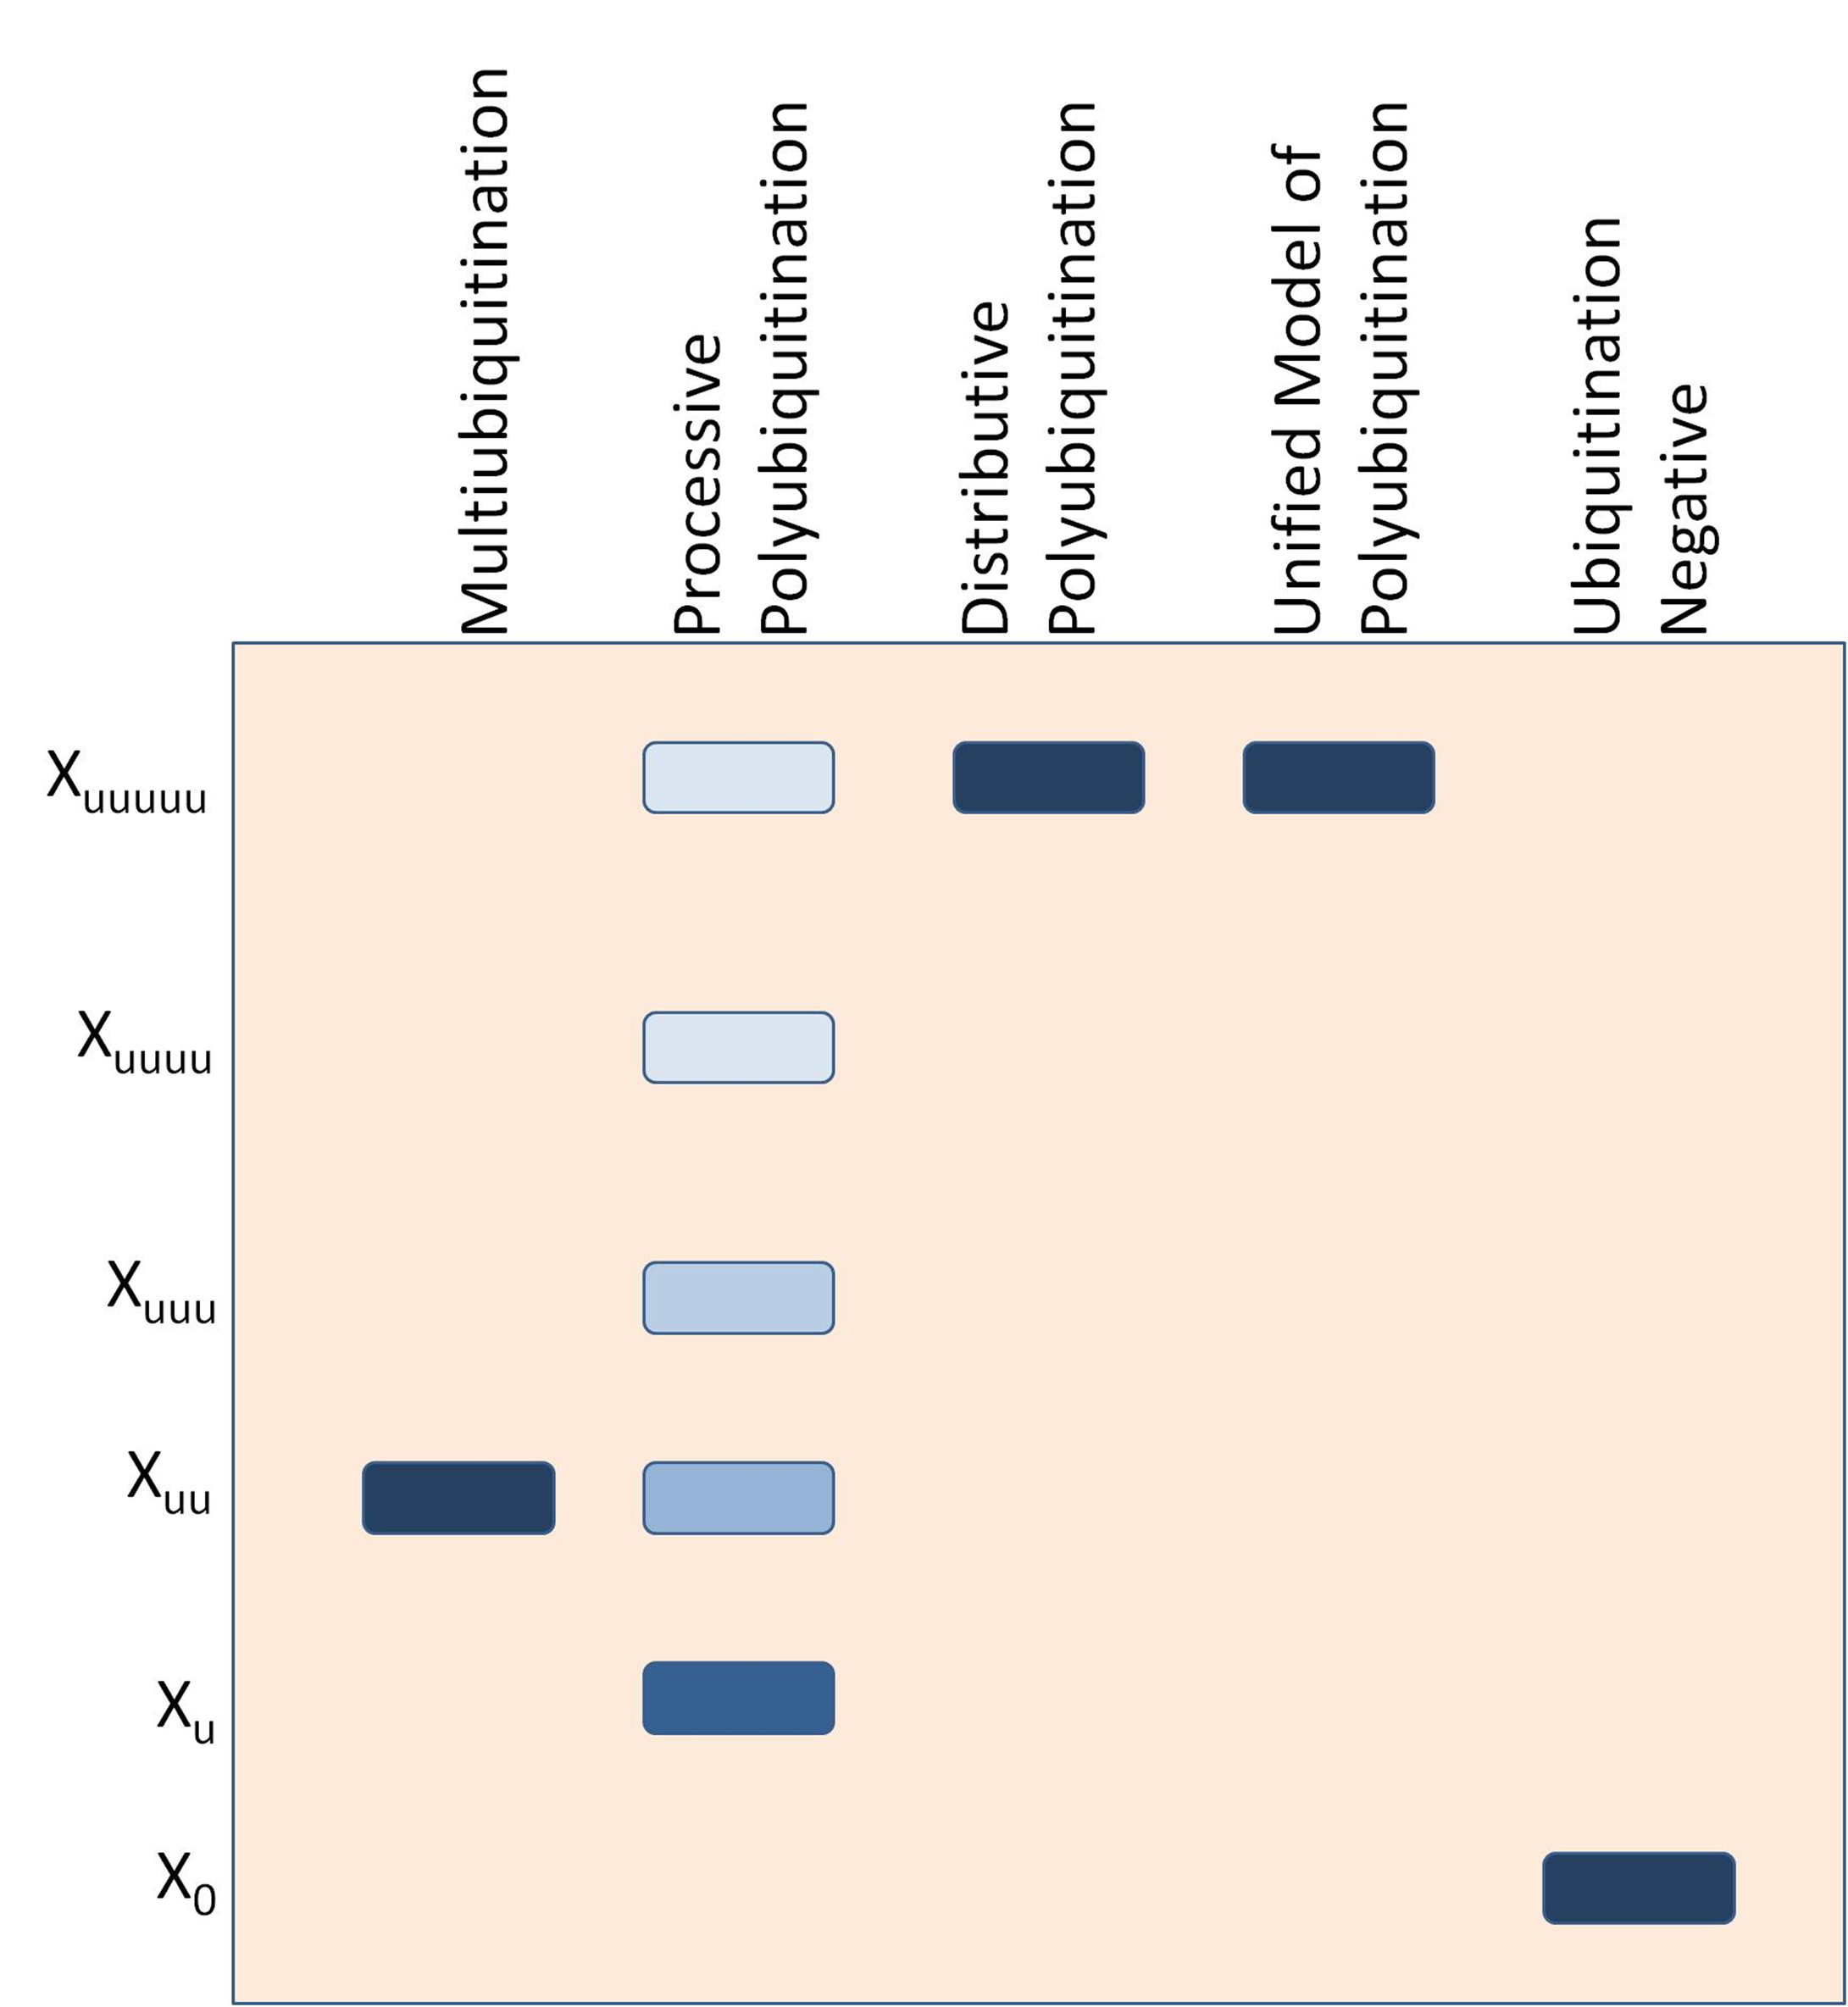
\includegraphics[width=1.0\textwidth]{./images/WB.png}
	\caption{Simulated Western blot of the model outputs, where all rate constants are equal to 1. The outputs of the models, shown in figures 2, 3, and 5, were used to predict the appearance of a Western blot containing samples from systems in which each form of ubiquitination investigated had taken place. A ubiquitination-negative sample was included as a negative control.}
	\label{fig:WB}
\end{figure}
}

One use of the models we have created is to determine from the final result of an experiment which form of ubiquitination has occurred. To determine the mode of ubiquitination, the protein levels in a sample must be determined. One way to determine protein levels in a sample is to perform a Western blot, where the proteins in the mixture are separated by size on a gel before being transferred to a membrane. Antibodies are incubated with the membrane and bind to the protein they were raised against. The visualisation of the binding of these antibodies allows the species present in a sample to be determined, along with their concentration relative to one another. A Western blot could indicate which form of ubiquitination has occurred. 

Figure~\ref{fig:WB} shows a predicted Western blot we have made for an experiment in which multiubiquitination, processive polyubiquitination, distributive polyubiquitination and unified polyubiquitination have all taken place, along with a ubiquitination negative control sample. We have predicted the appearance of this Western blot based on numerical solutions presented in sections ~\ref{multi}, ~\ref{distro}, ~\ref{proc} and ~\ref{unifed}.

Multiubiquitination, distributive polyubiquitination and unified polyubiquitination all lead to only one dark band being predicted as only one species is present. Processive polyubiquitination leads to a ladder of bands being predicted, with the higher molecular weight species giving progressively fainter bands. This is due to the sequentially lower concentrations of species as they progress through the simulation. This shows that while distributive polyubiquitination and the unified model of polyubiquitination cannot be distinguished from this Western blot, processive polyubiquitination, distributive polyubiquitination and multiubiquitination can be distinguished. However, we would be interested to know if this is true only for the parameters used herein.

\subsection{Sampling the Polyubiquitination Models}
\afterpage{
\begin{figure}[H]
	\centering
	\subfloat[Sampling k$_{1}$ between 0 and 25 in distributive polyubiquitination]{\label{fig:distro 0 25}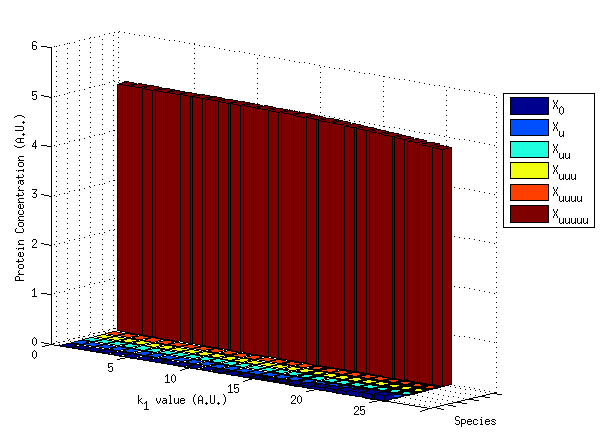
\includegraphics[width=0.48\textwidth]{./images/sampling/samplingdistributive0_25.png}}
	\hfill
	\subfloat[Sampling k$_{1}$ between 0 and 1000 in distributive polyubiquitination]{\label{fig:distro 0 1000}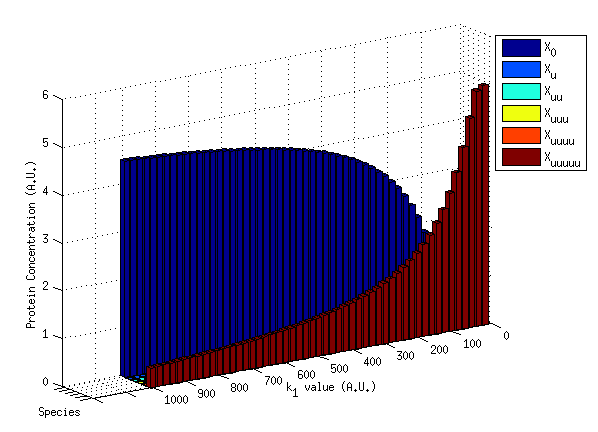
\includegraphics[width=0.48\textwidth]{./images/sampling/samplingdistributive0_1000.png}}

	\subfloat[Sampling k$_\text{off 0}$ between 0 and 25 in processive polyubiquitination]{\label{fig:proc 0 25}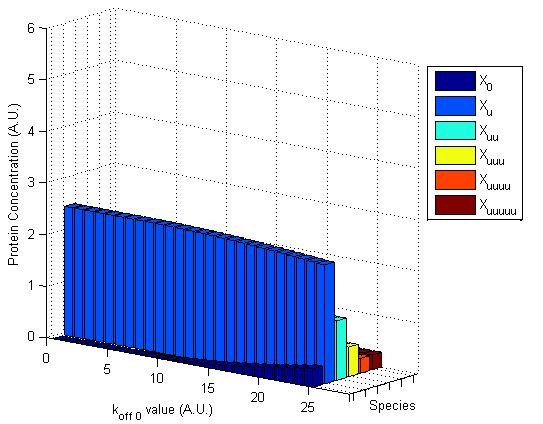
\includegraphics[width=0.48\textwidth]{./images/sampling/reprocessive0_25.png}}
	\hfill
	\subfloat[Sampling k$_\text{off 0}$ between 0 and 1000 in processive polyubiquitination]{\label{fig:proc 0 1000}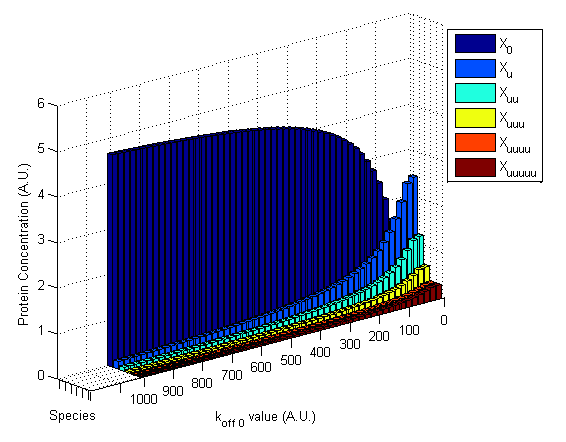
\includegraphics[width=0.48\textwidth]{./images/sampling/reprocessive0_1000.png}}

	\subfloat[Sampling k$_\text{off 0}$ between 0 and 25 in a unified model of polyubiquitination]{\label{fig:uni 0 25}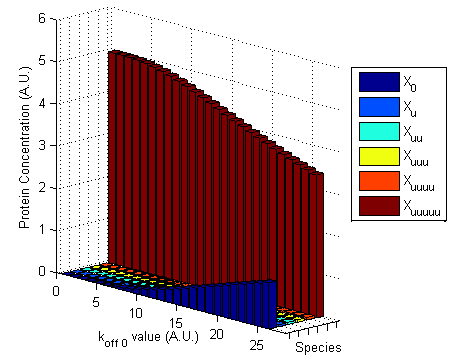
\includegraphics[width=0.48\textwidth]{./images/sampling/reunified0_25.png}}
	\hfill
	\subfloat[Sampling k$_\text{off 0}$ between 0 and 1000 in a unified model of polyubiquitination]{\label{fig:uni 0 1000}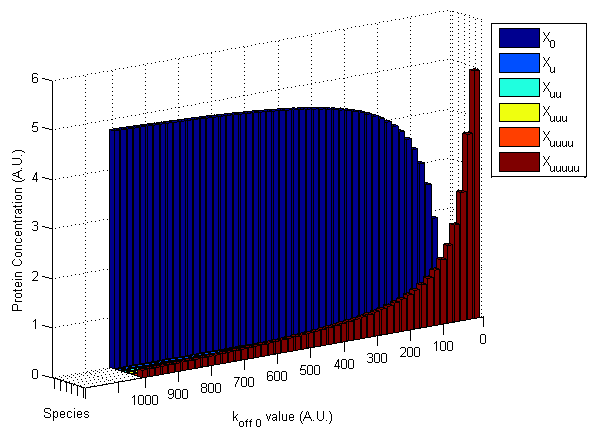
\includegraphics[width=0.48\textwidth]{./images/sampling/reunified0_1000.png}}

	\caption{Sampling the dissociation rate constants for the initial encounter between the ligase and unubiquitinated protein in models of polyubiquitination. The three models of polyubiquitination, a)-b) distributive (see appendix 2), c)-d) processive (see appendix 3) and e)-f) unified (see appendix 4), were all evaluated with a range of dissociation rate constants. Each plot shows the distribution of ubiquitin at steady state given a different dissociation rate. Each model was evaluated twice with rate constants between 0 and 25 in steps of 1 and between 0 and 1000 in steps of 20. The models were evaluated, and the final concentrations of each species was plotted.}
	\label{fig:Sampling}
\end{figure}
}

\afterpage{
\begin{figure}[H]
	\centering
	\subfloat[Sampling k$_{1}$ between 0 and 25 in processive polyubiquitination]{\label{fig:reproc 0 25}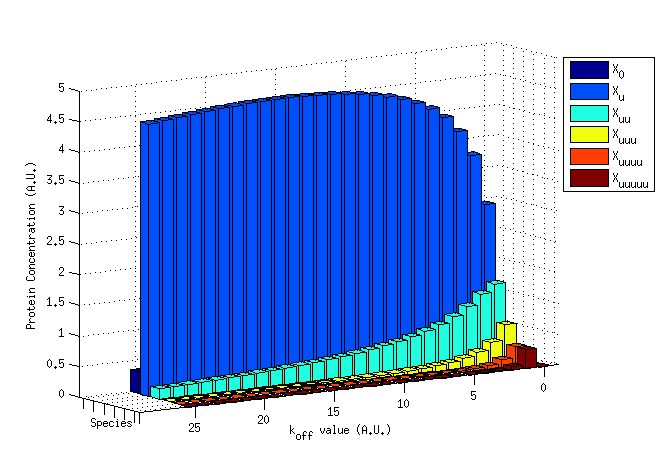
\includegraphics[width=0.48\textwidth]{./images/sampling/samplingprocessive0_25.png}}
	\hfill
	\subfloat[Sampling k$_{1}$ between 0 and 1000 in processive polyubiquitination]{\label{fig:reproc 0 1000}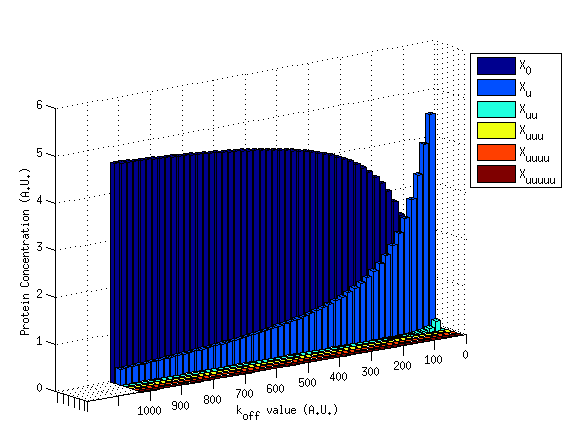
\includegraphics[width=0.48\textwidth]{./images/sampling/samplingprocessive0_1000.png}}

	\subfloat[Sampling k$_\text{off}$ between 0 and 25 in a unified model of polyubiquitination]{\label{fig:reuni 0 25}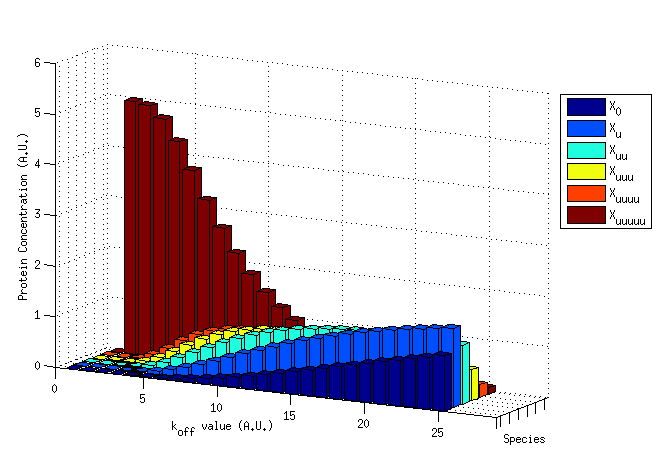
\includegraphics[width=0.48\textwidth]{./images/sampling/samplingunified0_25.png}}
	\hfill
	\subfloat[Sampling k$_\text{off}$ between 0 and 1000 in a unified model of polyubiquitination]{\label{fig:reuni 0 1000}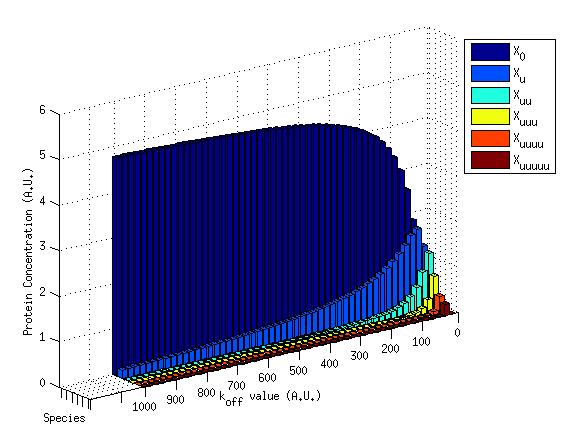
\includegraphics[width=0.48\textwidth]{./images/sampling/samplingunified0_1000.png}}

	\caption{Sampling the dissociation rate constants in models of polyubiquitination. The processive model of polyubiquitination (see appendix 3) and the unified model of polyubiquitination (see appendix 4) were modified such that all k$_\text{off}$ values were equal. The rate constants were then sampled. Each model was evaluated twice with rate constants between 0 and 25 in steps of 1 and between 0 and 1000 in steps of 20. The models were evaluated, and the final concentrations of each species was plotted.}
	\label{fig:reSampling}
\end{figure}
}

To investigate how the end state of our models of protein polyubiquitination change with rate constant, and to further investigate if the mode of polyubiquitination can be determined from observing the end state of the system, we sampled the dissociation constants of the three polyubiquitination models. The rates chosen for sampling were k$_1$ from the distributive model (see appendix 2), k$_\text{off 0}$ for the processive model (see appendix 3) and k$_\text{off 0}$ for the unified model (see appendix 4). These rates were chosen as we were attempting to replicate the \emph{in vivo} conditions. Data from Pierce at al\cite{pierce2009detection} shows that a high proportion of the substrate is unubiquitinated suggesting a high dissociation rate which regulates the pathway. Therefore the dissociation rates were of interest.

The sampling was implemented by solving the models with a series of values for the chosen rate. The ranges chosen were between 0 and 25 in steps of 1, and between 0 and 1000 in steps of 20. The models were solved, and the data were plotted. The results can be seen in figure~\ref{fig:Sampling}.

From these graphs, it is clear that the models behave in different ways upon sampling of the dissociation constants. The distributive model at lower k$_1$ values has high X$_{uuuuu}$ concentration. As k$_1$ increases, the level of X$_{uuuuu}$ decreases and X$_0$ increases. No other species is present at the end of the simulation. This shows that in this model, for k$_1$ values greater than 20, two species will be detectable if distributive polyubiquitination occurs.

In processive polyubiquitination, at low k$_\text{off 0}$ rates all substrate is ubiquitinated. Most substrate is monoubiquitinated and subsequent species have sequentially lower concentration. As k$_\text{off 0}$ increases, the level of X$_0$ increases gradually at the expense of the other species. Initially, the level of X$_u$ decreases. Subsequent species decrease at higher k$_\text{off 0}$ values.

The unified model of polyubiquitination resembles distributive polyubiquitination. At low k$_\text{off 0}$ values, all protein is in the X$_{uuuuu}$ state. As the k$_\text{off 0}$ value increases, the level of X$_0$ increases and the level of X$_{uuuuu}$ decreases. For most k$_\text{off 0}$ values, two protein species will be detectable. Therefore while processive polyubiquitination should be easily distinguishable from distributive and unified mechanisms of polyubiquitination, the distribuitve and unified mechanisms may be indistinguishable.

We investigated how the processive and unified models varied if all the k$_\text{off}$ rates were sampled simultaneously with the same value. This sampling was carried out as before, and the results can be seen in figure~\ref{fig:reSampling}. In processive polyubiquitination, at low k$_\text{off}$ rates all substrate is ubiquitinated. Most substrate is monoubiquitinated and subsequent species have sequentially lower concentration. As k$_\text{off}$ increases, the level of X$_u$ initially increases at the expense of other ubiquitinated protein species. X$_{uu}$ is the last ubiquitinated species other than X$_u$ to remain. This species eventually reaches zero before k$_\text{off}$ reaches 100. When k$_\text{off}$ is greater than 15, the concentration of X$_0$ starts to increase at the expense of X$_u$. As k$_\text{off}$ continues to increase, X$_0$ increases and X$_u$ decreases symmetrically. This shows that the number of species present at the end of a process if processive polyubiquitination is occuring varies with k$_\text{off}$.

In the unified model of polyubiquitination, at low k$_\text{off}$ values the only species present is X$_{uuuuu}$. As k$_\text{off}$ increases, the ubiquitinated species sequentially increase in concentration and X$_{uuuuu}$ decreases in concentration. All species other than X$_0$ eventually decrease; all except X$_u$ decrease to zero. X$_0$ increases with k$_\text{off}$. Similarly to the processive model, the species present at the end of the simulation depend on the k$_\text{off}$ value.

The unified model, with different combinations of parameters, results in a distribution of proteins similar to either the processive model or the distributive model. Figure~\ref{fig:reuni 0 1000} at high k$_\text{off}$ values resembles figures~\ref{fig:proc 0 1000} and~\ref{fig:reproc 0 1000}. The unified model results in figures~\ref{fig:uni 0 25} and~\ref{fig:uni 0 1000} at low and high k$_\text{off}$ values resemble the distributive models in figures~\ref{fig:distro 0 25} and~\ref{fig:distro 0 1000}. This implies that our unified model can represent both the processive and distributive models, given appropriate parameters.

\section{Discussion}

\subsection{Multiubiquitination}
Multiubiquitination is the addition of single ubiquitin monomers to multiple sites on the substrate protein by an E3 ligase. Figure~\ref{fig:multi model} shows a numerical solution for our model of this process, given in appendix 1. The simulation led to one species, multiubiquitinated protein. Figure~\ref{fig:WB} shows a simulated Western blot where we show the predicted appearance of reaction where multiubiquitination has occurred in the first lane.

The implications of the model are that if the system runs to thermodynamic equilibrium, only one species will be present. Therefore it can be determined if the process has reached its conclusion from analysing its makeup. This means that once a substrate protein enters this pathway, it is likely to be multiubiquitinated. Multiubiquitination is vital for the regulation of transport of proteins during internalisation\cite{monami2008grb10,staub2006role,mosesson2003endocytosis,haglund2003multiple}, and therefore its strict regulation is important: incorrectly internalised receptor proteins prevent proper cellular function. 

The regulation of this pathway may occur via kinetic proofreading\cite{hopfield1974kinetic}: a high k$_{1}$ rate in the initial encounter will lead to very few proteins being multiubiquitinated as it will be unlikely for a stable protein-ligase complex to form. However, if a protein is targeted for ubiquitination it could be altered by another modification such as phosphorylation. Phosphorylation is a post-translational modification which can mark proteins for ubiquitination. Phosphorylation leading to ubiquitination can depend on the presence of PEST domains\cite{yaglom1995p34cdc28,lanker1996rapid,kornitzer1994regulated} or can occur on single sites\cite{won1996activation,diehl1997inhibition}. This event could change the protein conformation, leading to altered binding to the ligase. This in turn could significantly lower the k$_{1}$ rate, allowing multiubiquitination to occur. The possibility of kinetic proofreading regulating this pathway should be investigated further by sampling the k$_{1}$ rate and investigating its impact on the entry of protein into the system.

A further avenue for future work is the interplay between k$_{2}$ and k$_6$. If one site is preferentially ubiquitinated over the other, its rate constant will be greater, leading to greater flux though that side of the pathway. Similarly interesting the concept of feedback: flux through the pathway may alter rate constants in the pathway, altering the fate of subsequent substrate. For example, the buildup of Y$^1_1$ may increase k$_3$. Another example is substrate level control of the rate of reaction. Mitogen-activated protein kinase phosphorylation has been shown to be regulated by substrate concentration \cite{kim2011substrate}. This could be implemented into our model.

\subsection{Polyubiquitination}
We investigated polyubiquitination, the construction of chains of ubiquitin on a single site of the substrate protein. We modelled both distributive and processive polyubiquitination (figure~\ref{fig:Polyubiquitination models}). The distributive polyubiquitination model led to a single protein species forming, X$_{uuuuu}$. This contrasted with the processive polyubiquitination model which resulted in a series of proteins with sequentially lower concentration as their point in the process increased. When the dissociation rate constants were sampled, see figure~\ref{fig:Sampling}, the results of the two models were distinct. The distributive and processive polyubiquitination models are distinct, both in terms of the composition of their results and the speed that the systems reached equilibrium. This is in keeping with the findings of Rape et al\cite{rape2006processivity} who showed that the processivity of a substrate determines how rapidly it is polyubiquitinated. When our model of processive polyubiquitination was compared to experimental results gained by Pierce et al\cite{pierce2009detection}, (see figure~\ref{fig:model v experimental}) the polyubiquitination of $\beta$-Cat and CYCE matched the model. This finding adds confidence to our model of processive polyubiquitination as it can return experimental results given the rate parameters.

Polyubiquitination can act as a form of kinetic proofreading\cite{hopfield1974kinetic}. In kinetic proofreading, multiple steps of a biological process have stringent kinetic parameters, meaning that it is highly unlikely for an unsuitable substrate to reach the end of a process. The kinetics of each reaction add a layer of stringency to a pathway beyond the signaling which leads to its activation. Only proteins with ubiquitin chains of length four or longer are recognised by the proteosome\cite{thrower2000recognition} and degraded. If the polyubiquitination process does not reach this key chain length, the proteosome does not read the protein as polyubiquitinated. As polyubiquitination involves multiple reversible reactions, each step represents an opportunity for the cell to proofread the process to ensure that only appropriate substrate is polyubiquitinated.

Polyubiquitination \emph{in vivo} occurs on a sliding scale of processivity\cite{rape2006processivity}. Some proteins are polyubiquitinated more processively and some more distributively.  Each reaction in polyubiquitination can have processive or distributive elements. The processivity of individual reactions determines the processivity of the overall process. In order to investigate the sliding scale of processivity, a unified model of polyubiquitination is presented (see figure~\ref{fig:Unified model}).

Sampling the models (see figures~\ref{fig:Sampling} and~\ref{fig:reSampling}) demonstrated that the unified model can resemble the distributive or processive models, depending on the rate constants chosen. This shows that the unified model encompasses both extremes of the processivity scale, and therefore can represent proteins which are at intermediate points on the scale. In the sampling experiment, very high k$_\text{off}$ values were chosen up to 1000 times the other rate constants. These high constants invariably resulted in most substrate protein being unubiquitinated. The biological relevance of these high constants is that if a protein is not marked for polyubiquitination, by phosphorylation or other mechanisms, the high k$_\text{off}$ rate for that protein prevents its polyubiquitination and subsequent degradation.

The discrete models of polyubiquitination we have presented impose an artificial structure on the process, whereas the unified model of polyubiquitination is closer to the continuum of processivity observed \emph{in vivo}. Therefore, it is more interesting for further study. One avenue for further investigation is which rates of reaction determine the processivity of the model: there may be important rate limiting steps which cause the overall process to be more or less processive. Similarly, the rate constants which are typical of processive or distributive polyubiquitination could be determined. Certain combinations of rate constants may impose a distributive or processive structure on the process, and these would be interesting to investigate further. Subsequently, there may be concentrations of protein in the final state of the system which imply that the process was more or less processive. Characterising the makeup of the system which is a hallmark of a certain degree of processivity would be instrumental in allowing the determination of the mechanism of polyubiquitination of real experimental results. It would allow the comparision of the processivity of different substrate proteins. The processivity determines how they compete for the ligase. This determines how rapidly they are polyubiquitinated and is important for substrate ordering.

The processivity of a substrate determines how it competes for the ligase. In our model we have not investigated the importance of the enzyme concentration. Modelling the ligase enzyme explicitly will be important for investigating competition between substrates for ligase, and the impact of this on ubiquitination.

If the model is further investigated, it may be possible to compare experimental results to the model and determine the mechanism of polyubiquitination as well as predict rate constants for the process under investigation. This would be a useful tool for molecular biologists investigating polyubiquitination. If the hallmark protein concentration trajectories for various levels of processivity were determined, experimental results could be compared to the model and their processivity could be predicted. If typical rate constants for different levels of processivity had been found, the rate constants for an experimental process could be predicted, giving laboratory scientists useful knowledge for further investigation. A further possibility would be the creation of a library of protein concentrations linked to the rate constants which resulted in this distribution, as well as where on the processivity scale the process sits. Experimental results could be compared to this library to predict rate constants and processivity levels.

A useful tool for life scientist working in polyubiquitination would be a user interface for the unified model of polyubiquitination which would allow each rate constant to be altered easily. The model would be evaluated and the output would be the resulting protein concentrations, which could be represented in a simulated Western blot. This would allow the investigator to predict how different rate constants affect the outcome, which would be useful for forming and testing hypotheses.

\section{Conclusion}
We have presented models for multiubiquitination, processive polyubiquitination, distributive polyubiquitination and a unified model for polyubiquitination. Polyubiquitination and multiubiquitination are distinct, as are processive and distributive polyubiquitination. These mechanisms of ubiquitination can be distinguished from one another. The unified model of polyubiquitination represents a more realistic continuum between the distributive and processive mechanisms of polyubiquitination, and should be investigated further.

\section{Appendices}
\appendix\renewcommand{\thesection}{\arabic{section}}
\section{Multiubiquitination Model}
Equations describing the model of multiubiquitination, where L is the E3 ligase and Y is the substrate protein. Y$_0$ is unubiquitinated protein, Y$^1$$_1$ is monoubiquitinated protein on site 1, Y$^2$$_1$ is monoubiquitinated protein on site 2, and Y$_2$ is multiubiquitinated protein. L.Y is a complex between the E3 ligase and the substrate protein Y.

\begin{align}
   Y_0 + L &\xrightleftharpoons[k_1]{k_0} L.Y_0 \\
  L.Y_0 \xrightarrow[]{k_2} L + Y^1_1
  &\xrightleftharpoons[k_4]{k_3} L.Y^1_1
  \xrightarrow[]{k_5} L + Y_2 \\
  L.Y_0 \xrightarrow[]{k_6} L + Y^2_1
  &\xrightleftharpoons[k_8]{k_7} L.Y^2_1
  \xrightarrow[]{k_9} L + Y_2
\end{align}

Ordinary differential equations:
\begin{align}
  \frac{\delta Y_0}{\delta t} &= k_1 L.Y_0 - k_0 Y_0 L \\
  \frac{\delta L.Y_0}{\delta t} &= k_0 Y_0 L - k_1 L.Y0 - k_2 L.Y_0 - k_6 L.Y_0 \\
  \frac{\delta Y^1_1}{\delta t}& = k_2 L.Y_0 + k_4 L.Y^1_1 - k_3 L Y^1_1\\
  \frac{\delta L.Y^1_1}{\delta t} &= k_3 L Y^1_1 - k_4 L.Y^1_1 - k_5 L.Y^1_1 \\
  \frac{\delta Y^2_1}{\delta t} &= k_6 L.Y_0 + k_8 L.Y^2_1 - k_7 L Y^2_1 \\
  \frac{\delta L.Y^2_1}{\delta t} &= k_7 L Y^2_1 - k_8 L.Y^2_1 - k_9 L.Y^2_1\\
  \frac{\delta Y_2}{\delta t} &= k_5 L.Y^1_1 + k_9 L.Y^2_1 
\end{align}

\section{Distributive Polyubiquitination Model}
Equations describing the model of distributive polyubiquitination, where L is the E3 ligase and X is the substrate protein. X$_0$ is unubiquitinated protein. X$_u$ is monoubiquitinated. The number of "u"s in the subscript denotes the number of ubiquitin monomers in the polyubiquitin chain. L.X is a complex between the E3 ligase L and the substrate protein X.

\begin{equation}
  X_0 + L \xrightleftharpoons[k_1]{k_0} L.X_0
  \xrightarrow[]{k_2} L + X_u
  \xrightleftharpoons[k_3]{k_4} L.X_u
  \xrightarrow[]{k_5} L + X_{uu}
  \xrightleftharpoons[k_6]{k_7} L.X_{uu}
  \xrightarrow[]{k_8} L + X_{uuu}
\end{equation}

\begin{equation}
  L + X_{uuu} \xrightleftharpoons[k_9]{k_{10}} L.X_{uuu}
  \xrightarrow[]{k_{11}} L + X_{uuuu}
  \xrightleftharpoons[k_{13}]{k_{12}} L.X_{uuuu}
  \xrightarrow[]{k_{14}} L + X_{uuuuu}
\end{equation}

Ordinary differential equations:
\begin{align}
  \frac{\delta X_0}{\delta t} &= k_1 L.X_0 - k_0 X_0 L \\
  \frac{\delta L.X_0}{\delta t} &= k_0 X_0 L - k_1 L.X_0 - k_2 L.X_0 \\
  \frac{\delta X_{u}}{\delta t} &= k_{2} L.X_{0} + k_{3} L.X_{u} - k_{4} X_{u} L\\
  \frac{\delta L.X_{u}}{\delta t} &= k_{4} X_{u} L - k_{3} L.X_{u} - k_{5} L.X_{u}\\
  \frac{\delta X_{uu}}{\delta t} &= k_{5} L.X_{u} + k_{6} L.X_{uu} - k_{7} X_{uu} L\\
  \frac{\delta L.X_{uu}}{\delta t} &= k_{7} X_{uu} L - k_{6} L.X_{uu} - k_{8} L.X_{uu} \\
  \frac{\delta X_{uuu}}{\delta t} &= k_{8} L.X_{uu} + k_{9} L.X_{uuu} - k_{10} X_{uuu} L\\
  \frac{\delta L.X_{uuu}}{\delta t} &= k_{10} X_{uuu} L - k_{9} L.X_{uuu} - k_{11} L.X_{uuu}\\
  \frac{\delta X_{uuuu}}{\delta t} &= k_{11} L.X_{uuu} + k_{13} L.X_{uuuu} - k_{12} X_{uuuu} L\\
  \frac{\delta L.X_{uuuu}}{\delta t} &= k_{12} X_{uuuu} L - k_{13} L.X_{uuuu} - k_{14} L.X_{uuuu}\\
  \frac{\delta X_{uuuuu}}{\delta t} &= k_{14} L.X_{uuuu}
\end{align}

\section{Processive Polyubiquitination}
Equations describing the  model of processive polyubiquitination, where L is the E3 ligase and X is the substrate protein.

\begin{equation}
  X_0 + L \xrightleftharpoons[k_\text{off 0}]{k_\text{on}} X_0.L
  \xrightarrow[]{k_0} X_u.L
  \xrightarrow[]{k_1} X_{uu}.L
  \xrightarrow[]{k_2} X_{uuu}.L
  \xrightarrow[]{k_3} X_{uuuu}.L
  \xrightarrow[]{k_4} X_{uuuuu}.L
\end{equation}

\begin{equation}
  X_u.L \xrightarrow[]{k_\text{off 1}} X_{u} + L
\end{equation}
\begin{equation}
  X_{uu}.L \xrightarrow[]{k_\text{off 2}} X_{uu} + L
\end{equation}
\begin{equation}
  X_{uuu}.L \xrightarrow[]{k_\text{off 3}} X_{uuu} + L
\end{equation}
\begin{equation}
  X_{uuuu}.L \xrightarrow[]{k_\text{off 4}} X_{uuuu} + L
\end{equation}
\begin{equation}
  X_{uuuuu}.L \xrightarrow[]{k_\text{off 5}} X_{uuuuu} + L
\end{equation}

Ordinary differential equations:
\begin{align}
  \frac{\delta X_0}{\delta t} &= k_\text{off 0} X_0.L - k_\text{on} X_0 L\\
  \frac{\delta X_{0}.L}{\delta t} &= k_\text{on} X_0 L - k_\text{off 0} X_0.L - k_0 X_0.L\\
  \frac{\delta X_{u}.L}{\delta t} &= k_0 X_{0}.L - k_\text{off 1} X_{u}.L - k_1 X_{u}.L\\
  \frac{\delta X_{u}}{\delta t} &= k_\text{off 1} X_{u}.L\\
  \frac{\delta X_{uu}.L}{\delta t} &= k_1 X_{u}.L - k_\text{off 2} X_{uu}.L - k_2 X_{uu}.L\\
  \frac{\delta X_{uu}}{\delta t} &= k_\text{off} X_{uu 2}.L\\
  \frac{\delta X_{uuu}.L}{\delta t} &= k_2 X_{uu}.L - k_\text{off 3} X_{uuu}.L - k_3 X_{uuu}.L\\
  \frac{\delta X_{uuu}}{\delta t} &= k_\text{off 3} X_{uuu}.L\\
  \frac{\delta X_{uuuu}.L}{\delta t} &= k_3 X_{uuu}.L - k_\text{off 4} X_{uuuu}.L - k_4 X_{uuuu}.L\\
  \frac{\delta X_{uuuu}}{\delta t} &= k_\text{off 4} X_{uuuu}.L\\
  \frac{\delta X_{uuuuu}.L}{\delta t} &= k_4 X_{uuuu}.L - k_\text{off 5} X_{uuuuu}.L\\
  \frac{\delta X_{uuuuu}}{\delta t} &= k_\text{off 5} X_{uuuuu}.L
\end{align}

\section{Unified Model of Polyubiquitination}
Equations describing the unified model of polyubiquitination, where L is the E3 ligase and X is the substrate protein.
\begin{equation}
  X_0 + L \xrightleftharpoons[k_\text{off 0}]{k_\text{on 0}} X_0.L
  \xrightarrow[]{k_0} X_u.L
  \xrightarrow[]{k_1} X_{uu}.L
  \xrightarrow[]{k_2} X_{uuu}.L
  \xrightarrow[]{k_3} X_{uuuu}.L
  \xrightarrow[]{k_4} X_{uuuuu}.L
\end{equation}
\begin{equation}
  X_u.L \xrightleftharpoons[k_\text{on 1}]{k_\text{off 1}} X_{u} + L
\end{equation}
\begin{equation}
  X_{uu}.L \xrightleftharpoons[k_\text{on 2}]{k_\text{off 2}} X_{uu} + L
\end{equation}
\begin{equation}
  X_{uuu}.L \xrightleftharpoons[k_\text{on 3}]{k_\text{off 3}} X_{uuu} + L
\end{equation}
\begin{equation}
  X_{uuuu}.L \xrightleftharpoons[k_\text{on 4}]{k_\text{off 4}} X_{uuuu} + L
\end{equation}
\begin{equation}
  X_{uuuuu}.L \xrightarrow[]{k_\text{off 5}} X_{uuuuu 5} + L
\end{equation}

Ordinary differential equations:
\begin{align}
  \frac{\delta X_0}{\delta t} &= k_\text{off 0} X_0.L - k_\text{on 0} X_0  L\\
  \frac{\delta X_{0}.L}{\delta t} &= k_\text{on 0} X_0  L - k_\text{off 0} X_0.L - k_0 X_0.L\\
  \frac{\delta X_{u}.L}{\delta t} &= k_0 X_{0}.L + k_\text{on 1} X_{u}  L - k_1 X_{u}.L - k_\text{off 1} X_{u}.L\\
  \frac{\delta X_{uu}.L}{\delta t} &= k_1 X_{u}.L + k_\text{on 2} X_{uu}  L - k_2 X_{uu}.L - k_\text{off 2} X_{uu}.L\\
  \frac{\delta X_{uuu}.L}{\delta t} &= k_2 X_{uu}.L + k_\text{on 3} X_{uuu}  L - k_3 X_{uuu}.L - k_\text{off 3} X_{uuu}.L\\
  \frac{\delta X_{uuuu}.L}{\delta t} &= k_3 X_{uuu}.L + k_\text{on 4} X_{uuuu}  L - k_4 X_{uuuuu}.L - k_\text{off 4} X_{uuuu}.L\\
  \frac{\delta X_{uuuuu}.L}{\delta t} &= k_4 X_{uuuu}.L - k_\text{off 5} X_{uuuuu}.L\\
  \frac{\delta X_{u}}{\delta t} &= k_\text{off 1} X_{u}.L - k_\text{on 1} X_{u}  L\\
  \frac{\delta X_{uu}}{\delta t} &= k_\text{off 2} X_{uu}.L - k_\text{on 2} X_{uu}  L\\
  \frac{\delta X_{uuu}}{\delta t} &= k_\text{off 3} X_{uuu}.L - k_\text{on 3} X_{uuu} L\\
  \frac{\delta X_{uuuu}}{\delta t} &= k_\text{off 4} X_{uuuu}.L - k_\text{on 4} X_{uuuu}  L\\
  \frac{\delta X_{uuuuu}}{\delta t} &= k_\text{off 5} X_{uuuuu}.L
\end{align}

\bibliographystyle{unsrt}
\bibliography{references}

\end{document}